%%%%%%%%%%%%%%%%%%%%%%%%%%%%%%%%%%%%%%%%%%%%%%%%%%%%%%%%%%%%%%%%%%%%%%%%%%%%%%%%%%%%%%%%
% Setup I6pd2 style, common packages
%%%%%%%%%%%%%%%%%%%%%%%%%%%%%%%%%%%%%%%%%%%%%%%%%%%%%%%%%%%%%%%%%%%%%%%%%%%%%%%%%%%%%%%%
\documentclass[final,hyperref={pdfpagelabels=false},noamsthm]{beamer}
\usepackage{default}

\usetheme{I6pd2} % Use the I6pd2 theme supplied with this template

\usepackage[english]{babel} % English language/hyphenation

\usepackage{amsmath,amsthm}
\usepackage{multirow}
\usepackage{makecell}

\usepackage{tikz}
\usetikzlibrary{fit}					% fitting shapes to coordinates
\usetikzlibrary{backgrounds}	% drawing the background after the foreground

%%%%%%%%%%%%%%%%%%%%%%%%%%%%%%%%%%%%%%%%%%%%%%%%%%%%%%%%%%%%%%%%%%%%%%%%%%%%%%%%%%%%%%%%
% Shortcuts for this project
%%%%%%%%%%%%%%%%%%%%%%%%%%%%%%%%%%%%%%%%%%%%%%%%%%%%%%%%%%%%%%%%%%%%%%%%%%%%%%%%%%%%%%%%

% blackboard series
\def\bbP{\mathbb{P}}
\def\bbp{\mathbb{p}}
\def\bbE{\mathbb{E}}
\def\bbN{\mathbb{N}}

% calligraphic series
\def\calT{\mathcal{T}}
\def\calW{\mathcal{W}}
\def\calX{\mathcal{X}}

% bold series
\def\bfP{\mathbf{P}}
\def\bfX{\mathbf{X}}

% distributions
\def\aDist{\Lambda}
\def\aTime{T}
\def\Geom{\text{Geom}}

% stuff
\newcommand{\prob}{\mathbb{P}}
\newcommand{\calV}{\mathcal{V}}
\newcommand{\calE}{\mathcal{E}}
\newcommand{\ee}{Z} % ends of edges
\newcommand{\bfee}{\mathbf{\ee}}
\newcommand{\bfE}{\mathbf{E}}
\newcommand{\PYP}{\mathcal{PYP}}
\newcommand{\geom}{\beta}
\newcommand{\BNTL}{\text{\rm BNTL}}
\newcommand{\bfT}{\mathbf{T}}
\newcommand{\calO}{\mathcal{O}}
\newcommand{\bbR}{\mathbb{R}}
\newcommand{\bfPsi}{\boldsymbol{\Psi}}
\newcommand{\bfn}{\mathbf{n}}
\newcommand{\bfd}{\mathbf{d}}
\newcommand{\argdot}{{\,\vcenter{\hbox{\scalebox{0.5}{$\bullet$}}}\,}}%{\bullet}
\def\indicator{\mathbf{1}}
\newcommand{\limscale}[2]{\overset{\scriptscriptstyle{#1 \uparrow #2}}{\widesim[1.25]}}
\newcommand{\simiid}{\overset{\scriptscriptstyle{\text{i.i.d.}}}{\widesim}}
\newcommand{\widesim}[1][1.5]{
	\mathrel{\scalebox{#1}[1]{$\sim$}}
}

%%%%%%%%%%%%%%%%%%%%%%%%%%%%%%%%%%%%%%%%%%%%%%%%%%%%%%%%%%%%%%%%%%%%%%%%%%%%%%%%%%%%%%%%
% Define footer contents
%%%%%%%%%%%%%%%%%%%%%%%%%%%%%%%%%%%%%%%%%%%%%%%%%%%%%%%%%%%%%%%%%%%%%%%%%%%%%%%%%%%%%%%%

\newcommand{\leftfoot}{} % Left footer text

\newcommand{\rightfoot}{~ \url{http://csml.stats.ox.ac.uk/learning/}} % Right footer text


\title{Sampling and Inference for Beta Neutral-to-the-Left Models of Sparse Networks} % Poster title

\author{Benjamin Bloem-Reddy, \underline{Adam Foster}, Emile Mathieu, Yee Whye Teh }
\institute{Department of Statistics, University of Oxford}

%%%%%%%%%%%%%%%%%%%%%%%%%%%%%%%%%%%%%%%%%%%%%%%%%%%%%%%%%%%%%%%%%%%%%%%%%%%%%%%%%%%%%%%%
% Main presentation
%%%%%%%%%%%%%%%%%%%%%%%%%%%%%%%%%%%%%%%%%%%%%%%%%%%%%%%%%%%%%%%%%%%%%%%%%%%%%%%%%%%%%%%%

\begin{document}
	
\begin{frame}[plain]
	\titlepage
\end{frame}

\begin{frame}
	\frametitle{Contents}
	\tableofcontents
\end{frame}

\section{Background}

\begin{frame}
	\frametitle{Temporal networks}
	\textbf{Example}
	\begin{itemize}
		\item Messages sent between people over time
		\item Protein-protein interactions
	\end{itemize}
	
\end{frame}

\begin{frame}
	\frametitle{Temporal networks}
	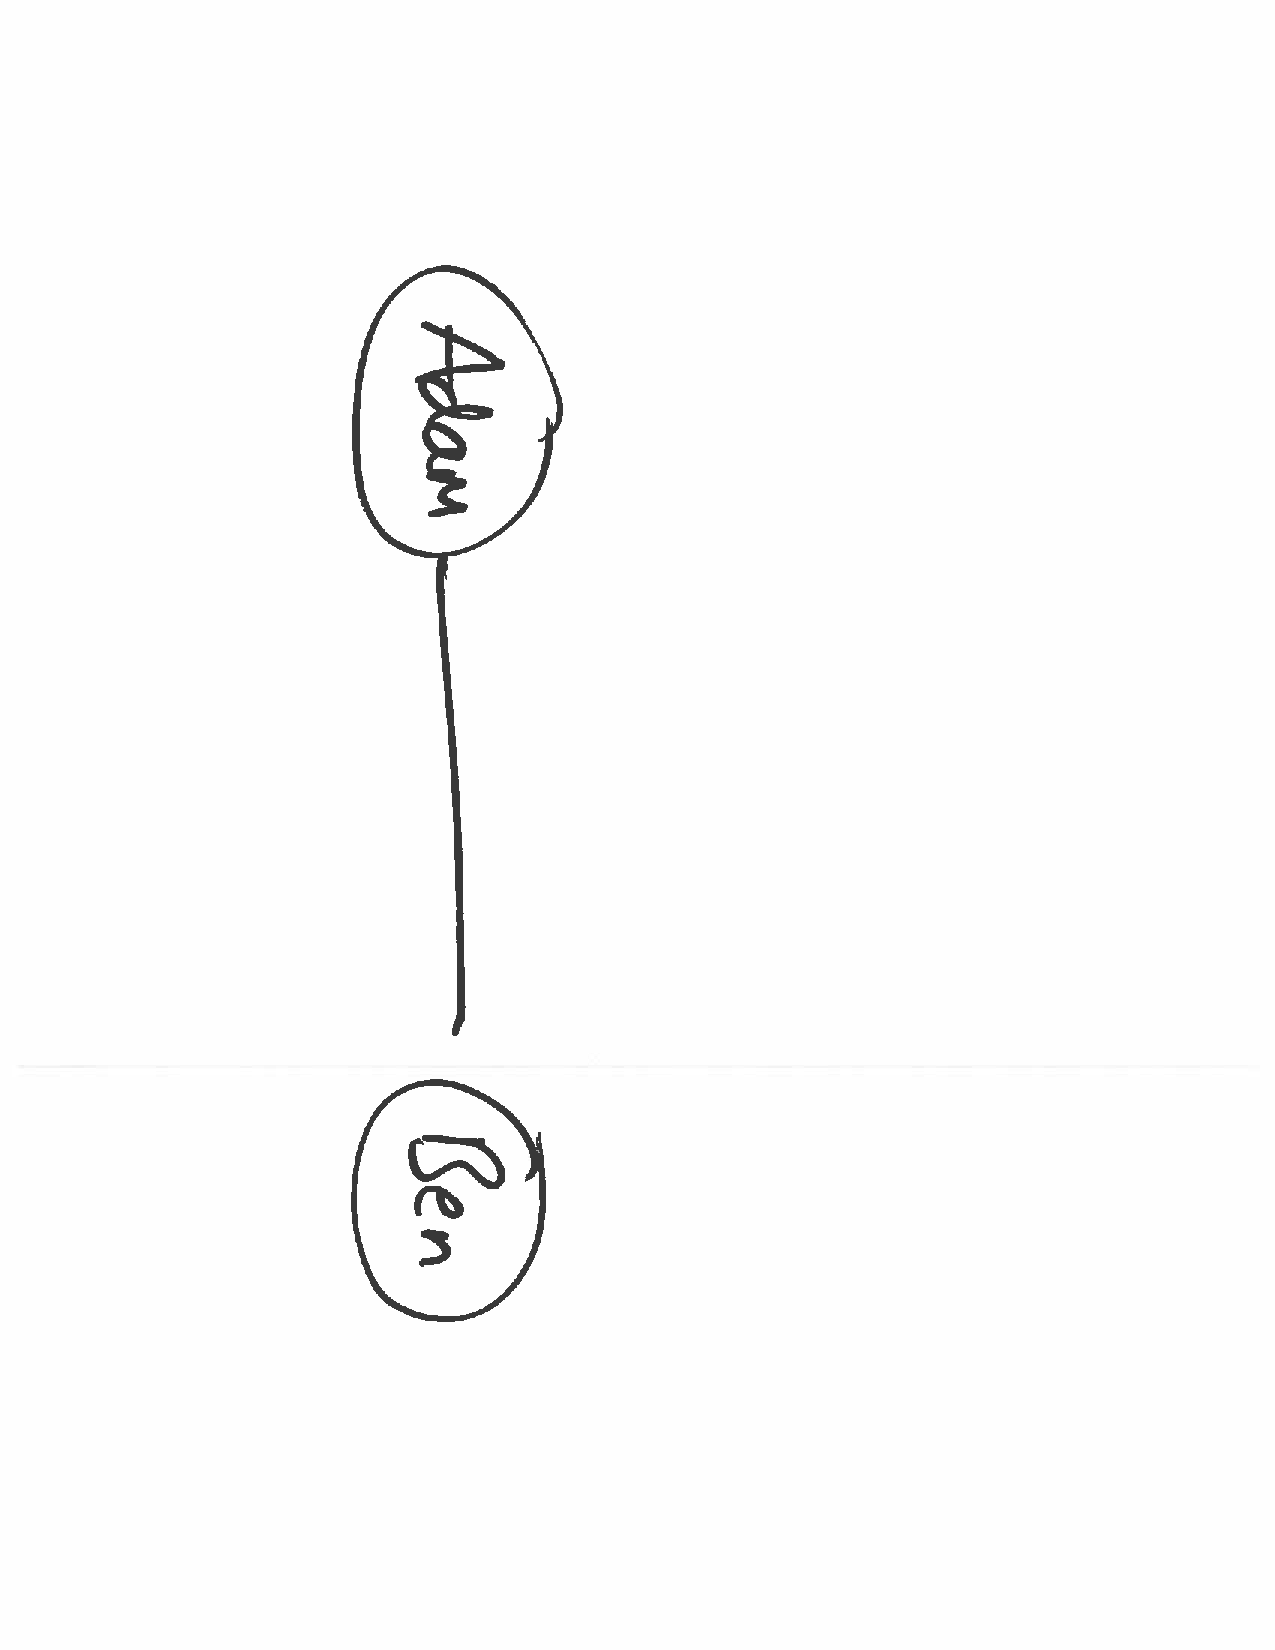
\includegraphics[angle=90,origin=c,scale=0.4]{fig/socialnet1}
\end{frame}

\begin{frame}
	\frametitle{Temporal networks}
	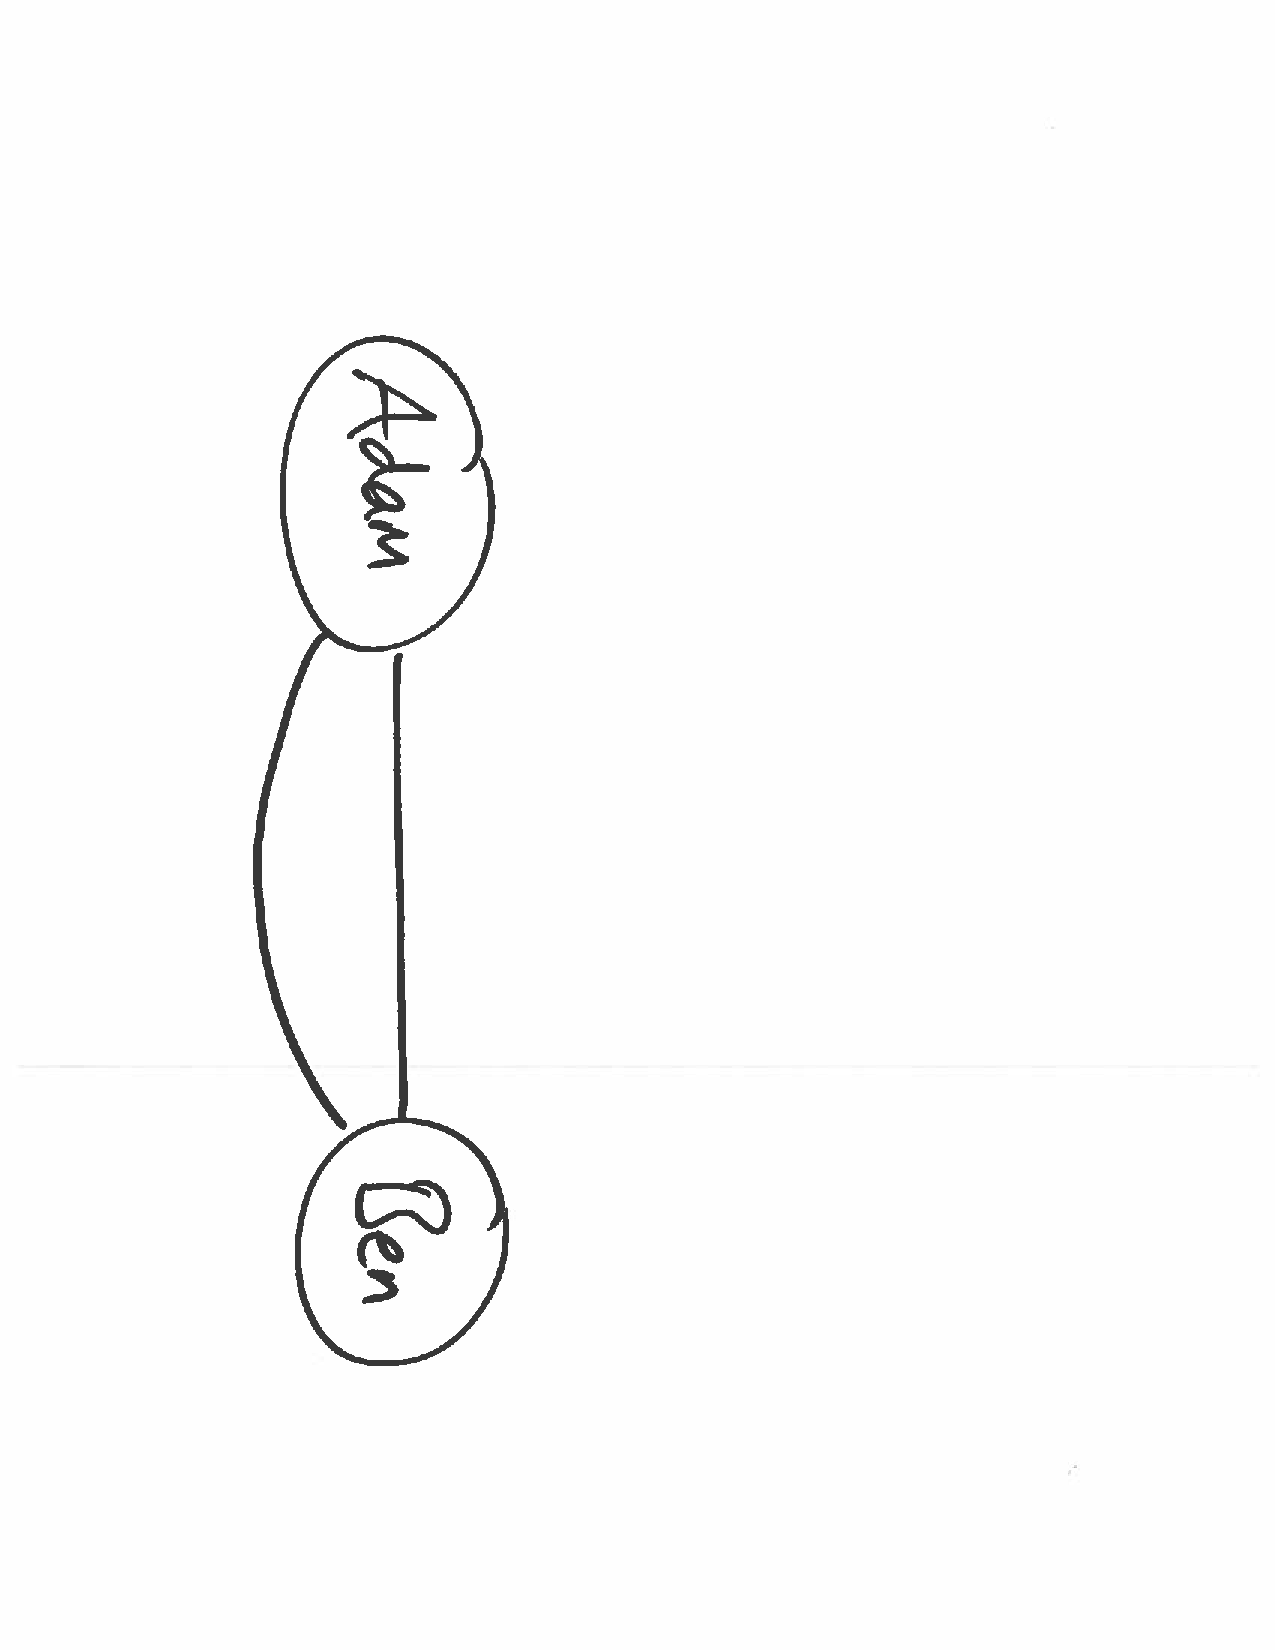
\includegraphics[angle=270,origin=c,scale=0.4]{fig/socialnet2}
\end{frame}

\begin{frame}
	\frametitle{Temporal networks}
	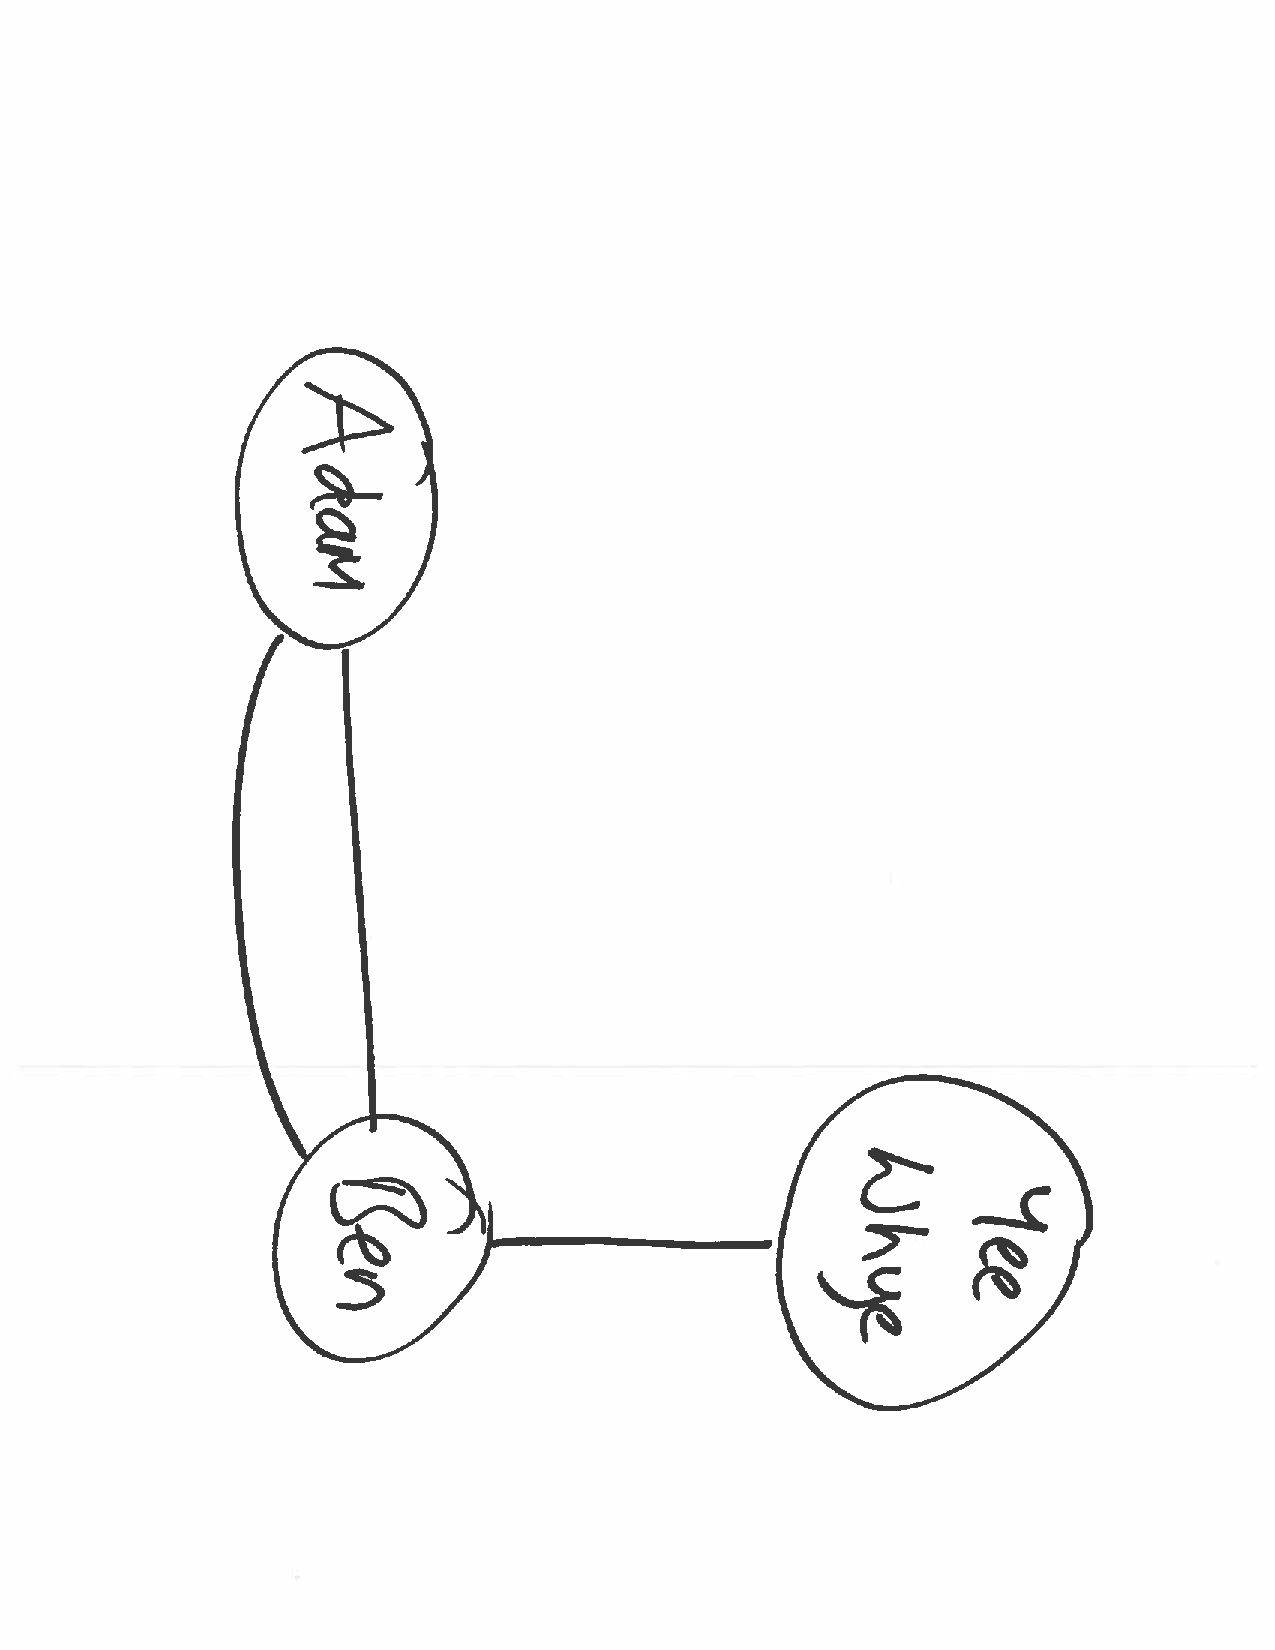
\includegraphics[angle=90,origin=c,scale=0.4]{fig/socialnet3}
\end{frame}

\begin{frame}
	\frametitle{Temporal networks}
	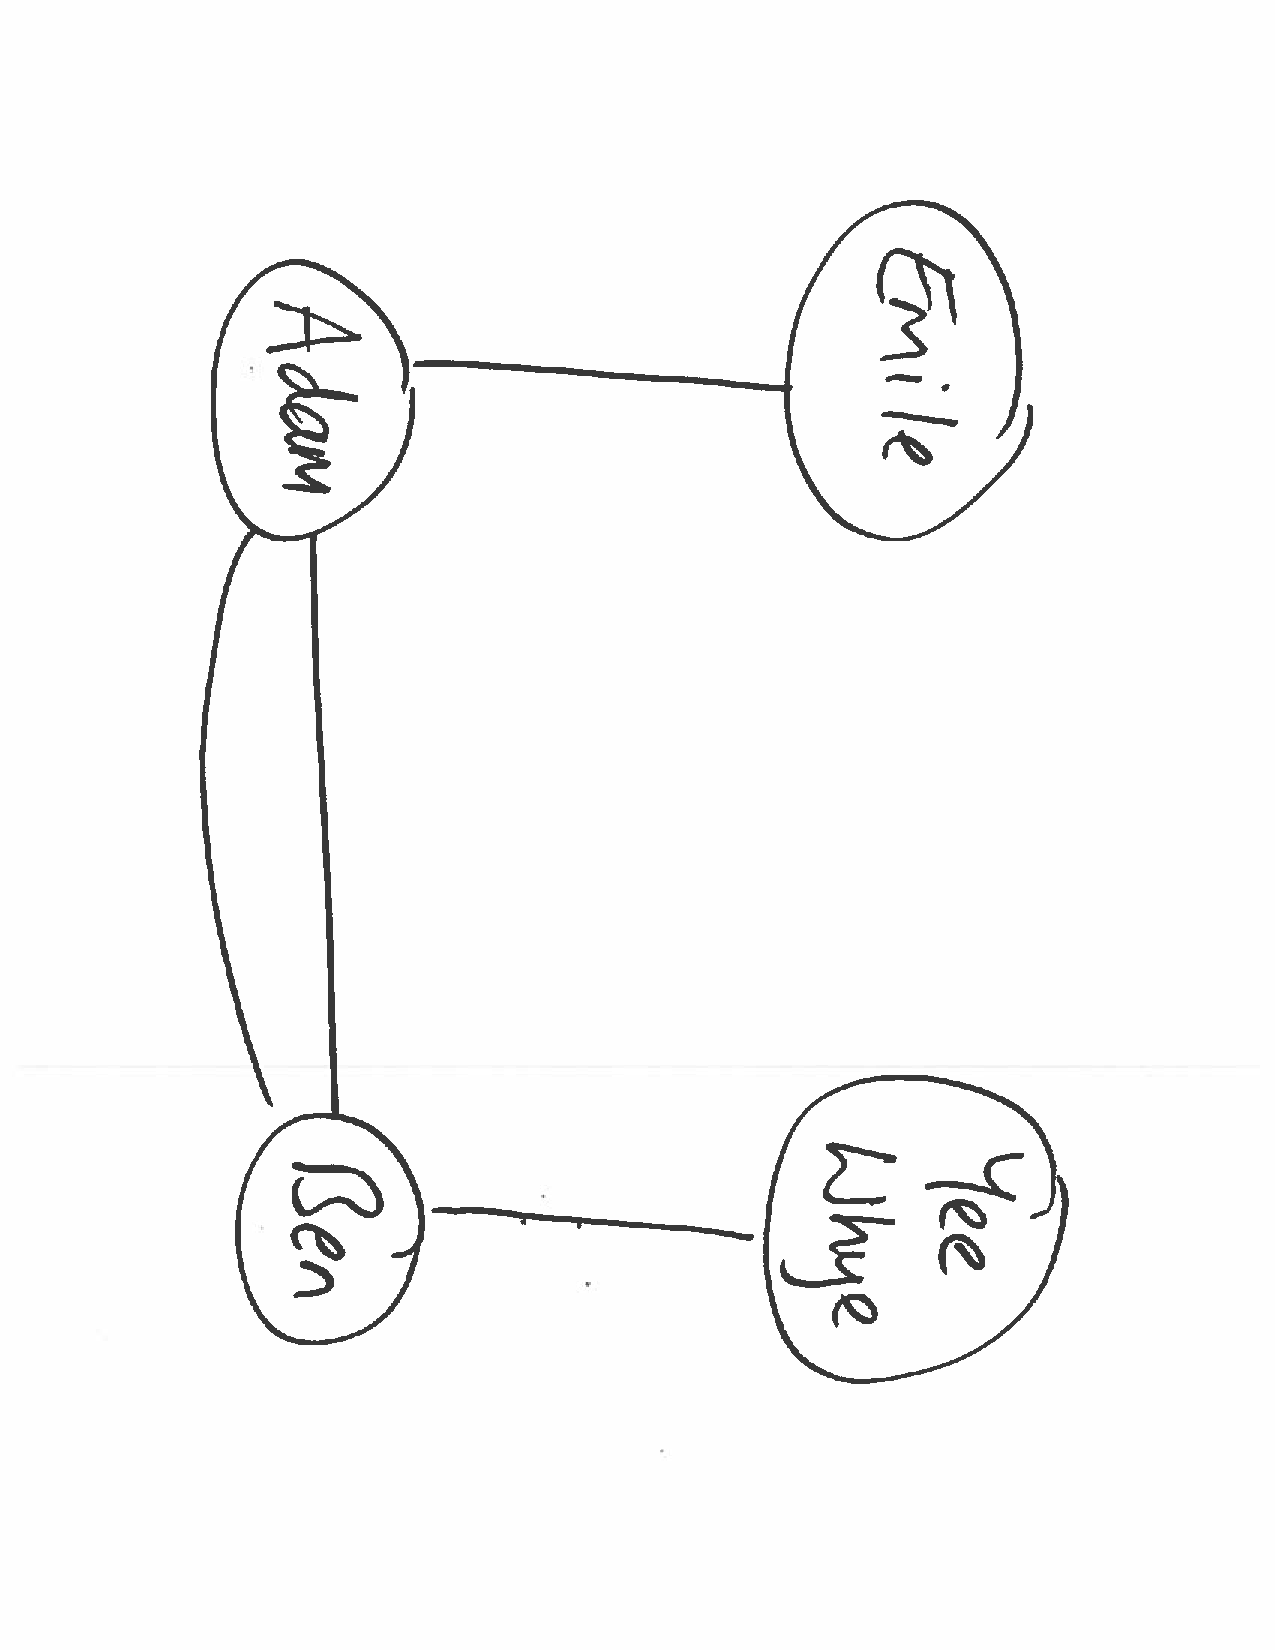
\includegraphics[angle=90,origin=c,scale=0.4]{fig/socialnet4}
\end{frame}

\begin{frame}
	\frametitle{Edges and vertices}
	TODO: break picture into 4
	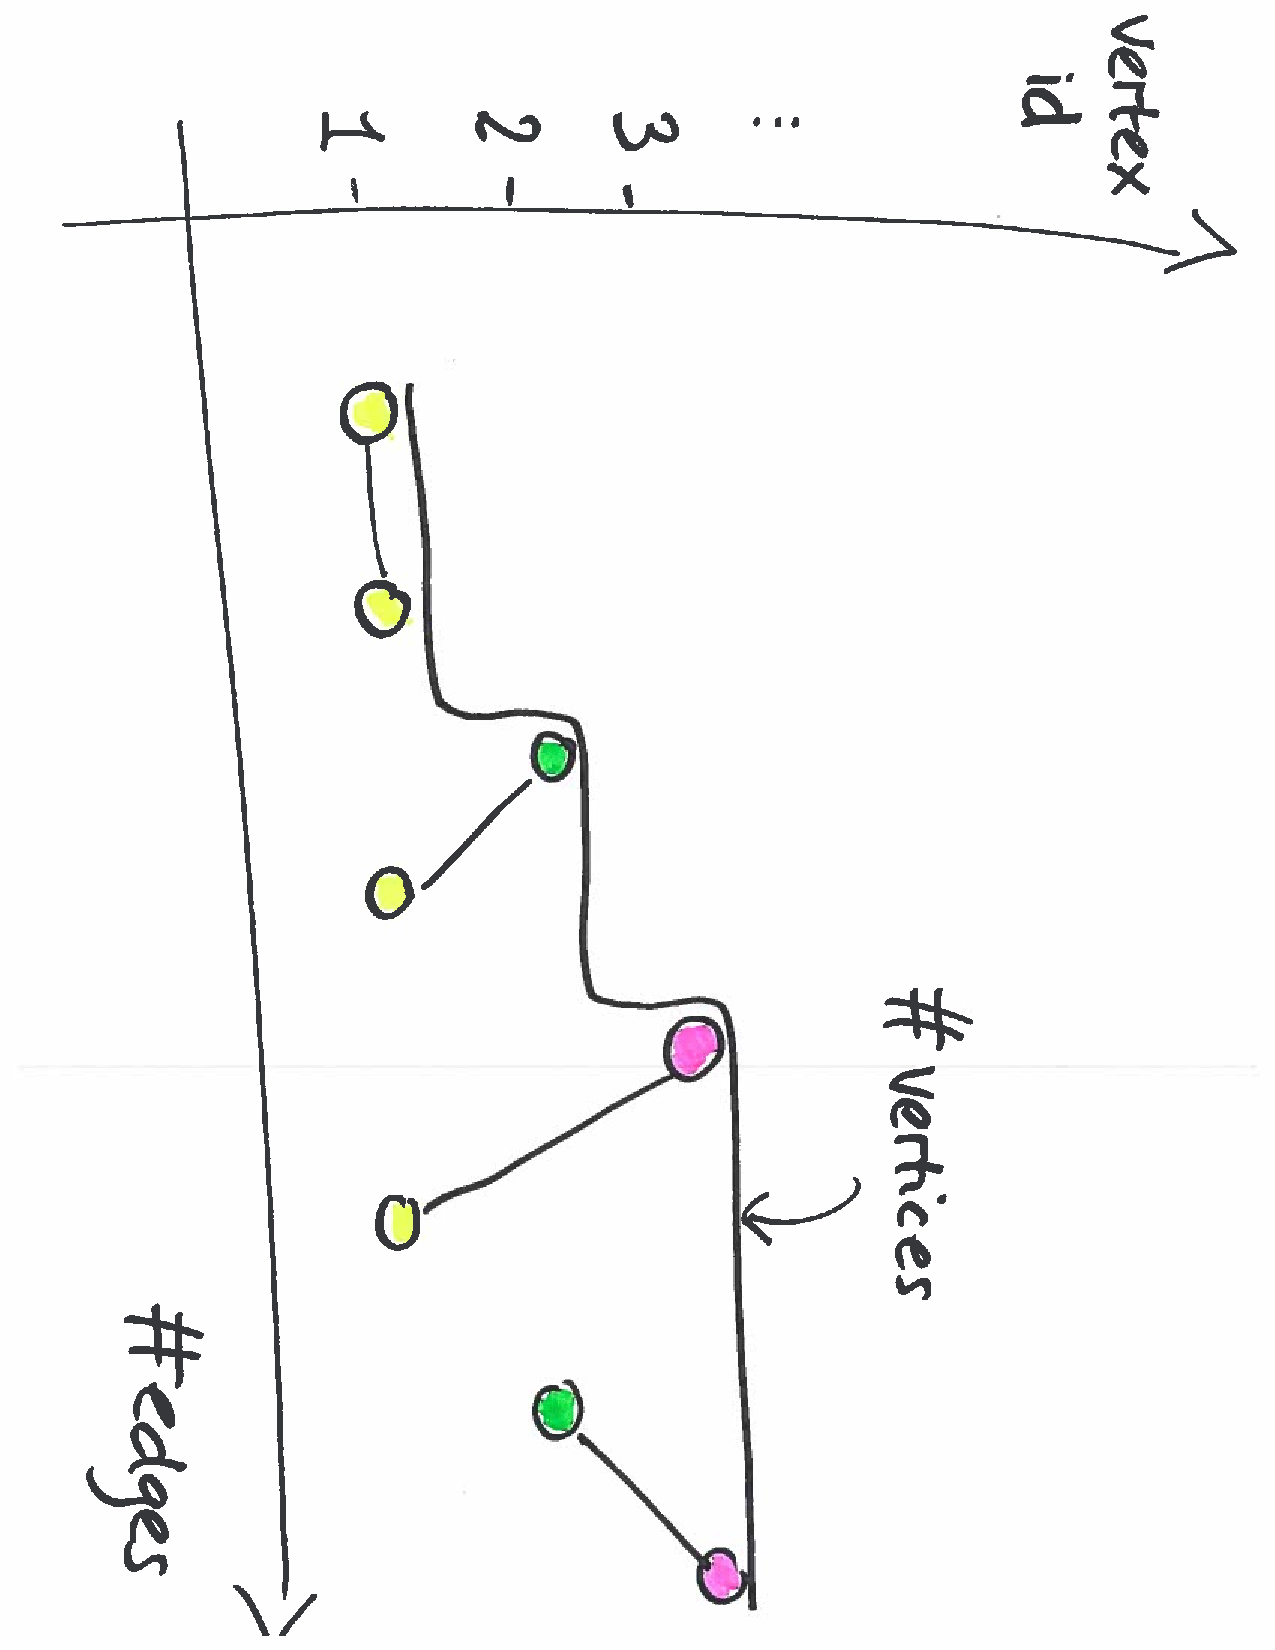
\includegraphics[angle=90,origin=c,scale=0.4]{fig/edgevertex}
\end{frame}


\begin{frame}
	\frametitle{Sparsity}
	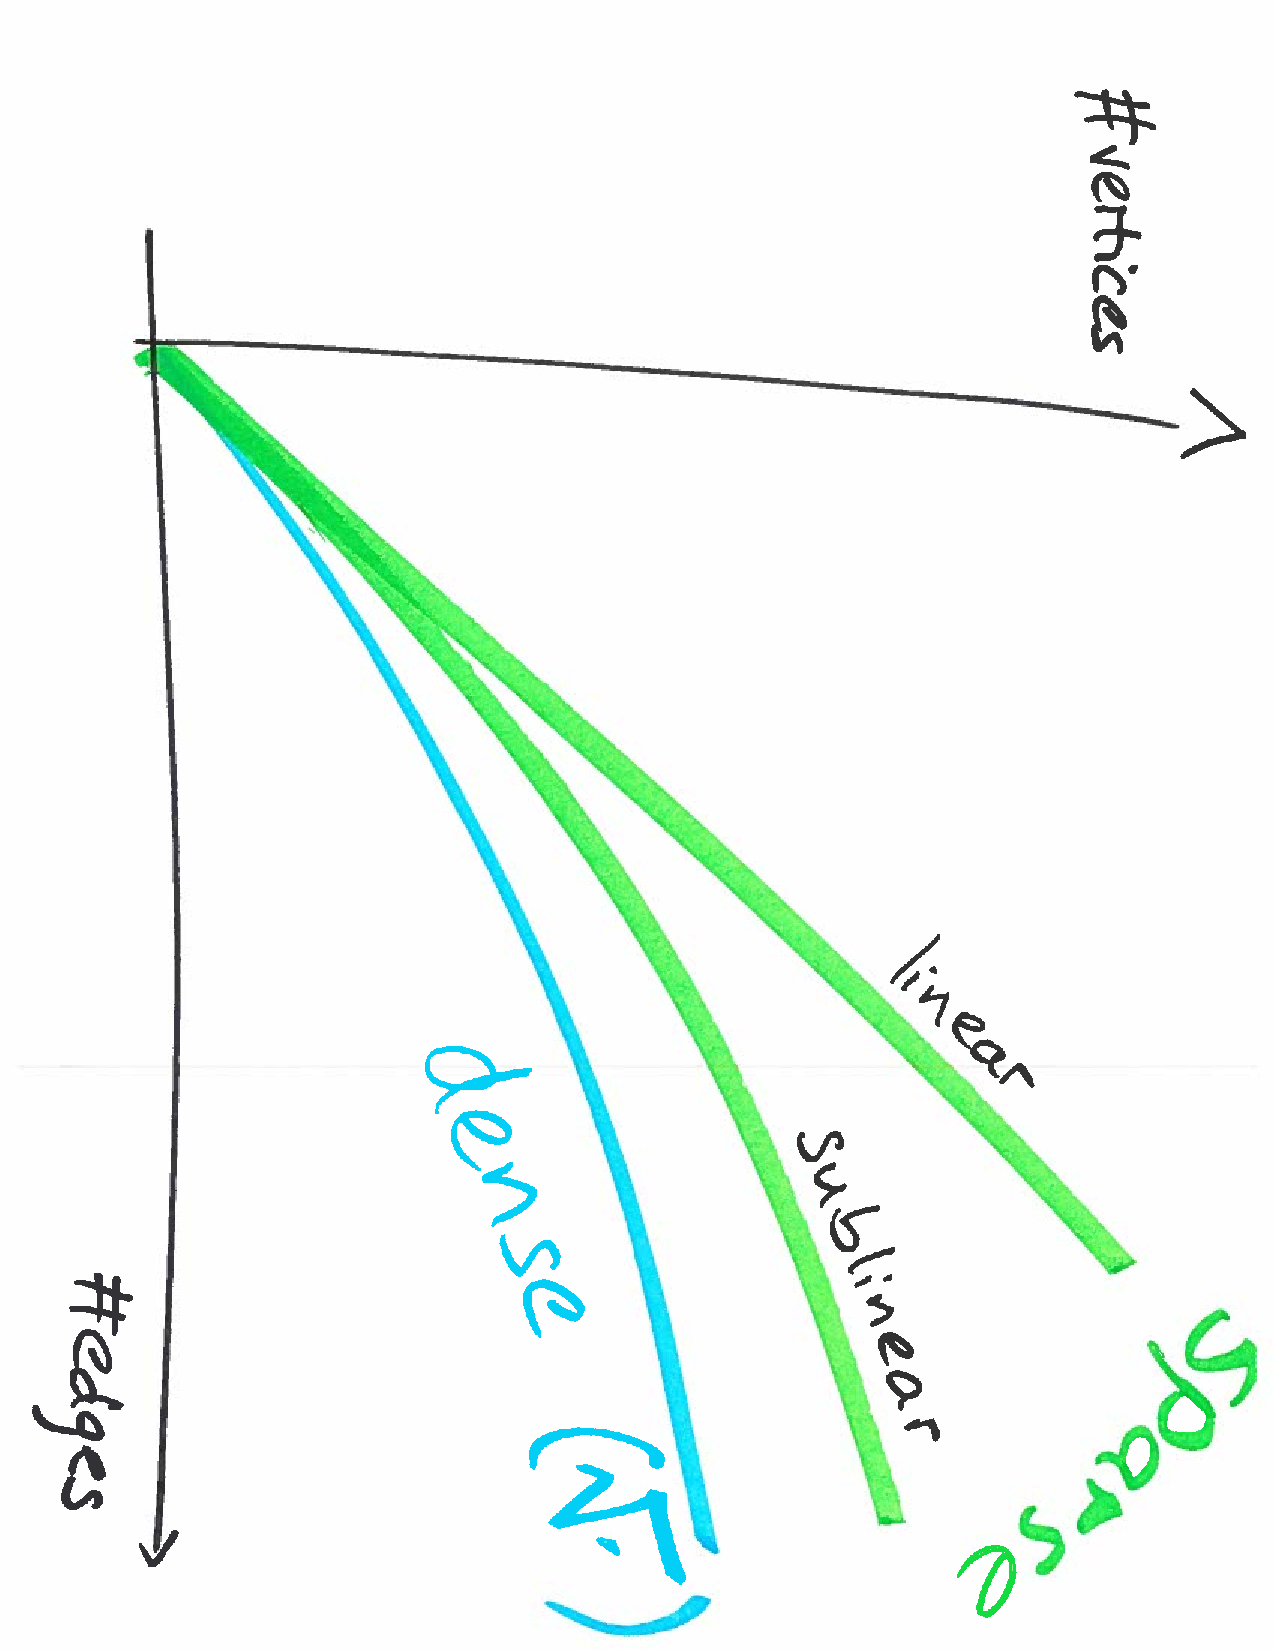
\includegraphics[angle=90,origin=c,scale=0.4]{fig/sparsity}
\end{frame}

\begin{frame}
	\frametitle{Power law degree distribution}
	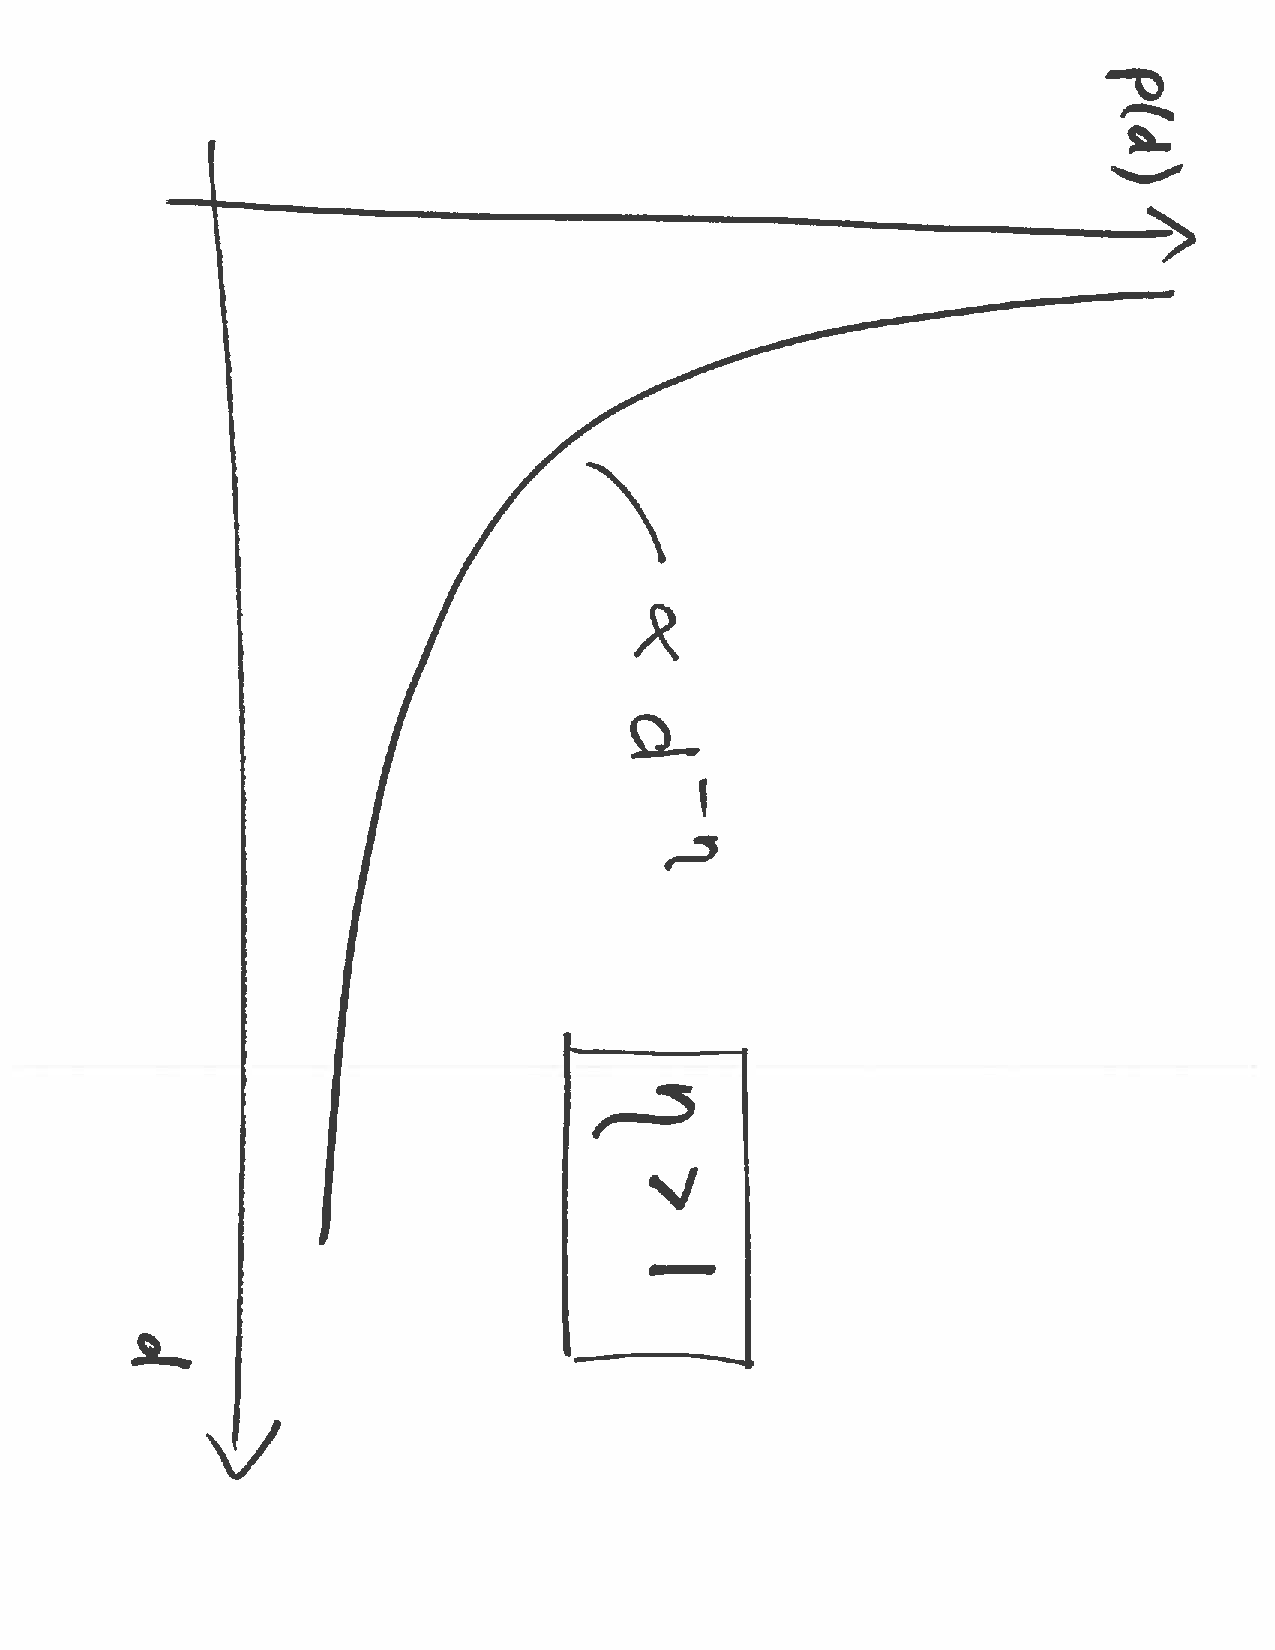
\includegraphics[angle=90,origin=c,scale=0.37]{fig/powerlaw}
\end{frame}

\begin{frame}
	\frametitle{Sparsity and power law}
	\begin{align*}
	\textbf{Sublinear } \text{sparsity} & \quad \iff \quad  \eta \in (1,2) \\
	\textbf{Linear } \text{sparsity} & \quad \iff \quad \eta > 2
	\end{align*}
\end{frame}

\begin{frame}
	\frametitle{Empirical study}
	\begin{table}[b]
		% \vspace*{-\baselineskip}
		\label{tab:datasets}
		\begin{center}
			\begin{tabular}{lll}
				SNAP dataset \cite{snapnets} & \# of vertices   & \# of edges    \\
				\hline
				Ask Ubuntu    & 159,316   & 964,437    \\
				UCI social network   & 1,899     & 20,296     \\
				\vdots & \vdots & \vdots
			\end{tabular}
		\end{center}
	\end{table}
	
\end{frame}

\begin{frame}
	\frametitle{Ask Ubuntu}
	\begin{figure}[h]
		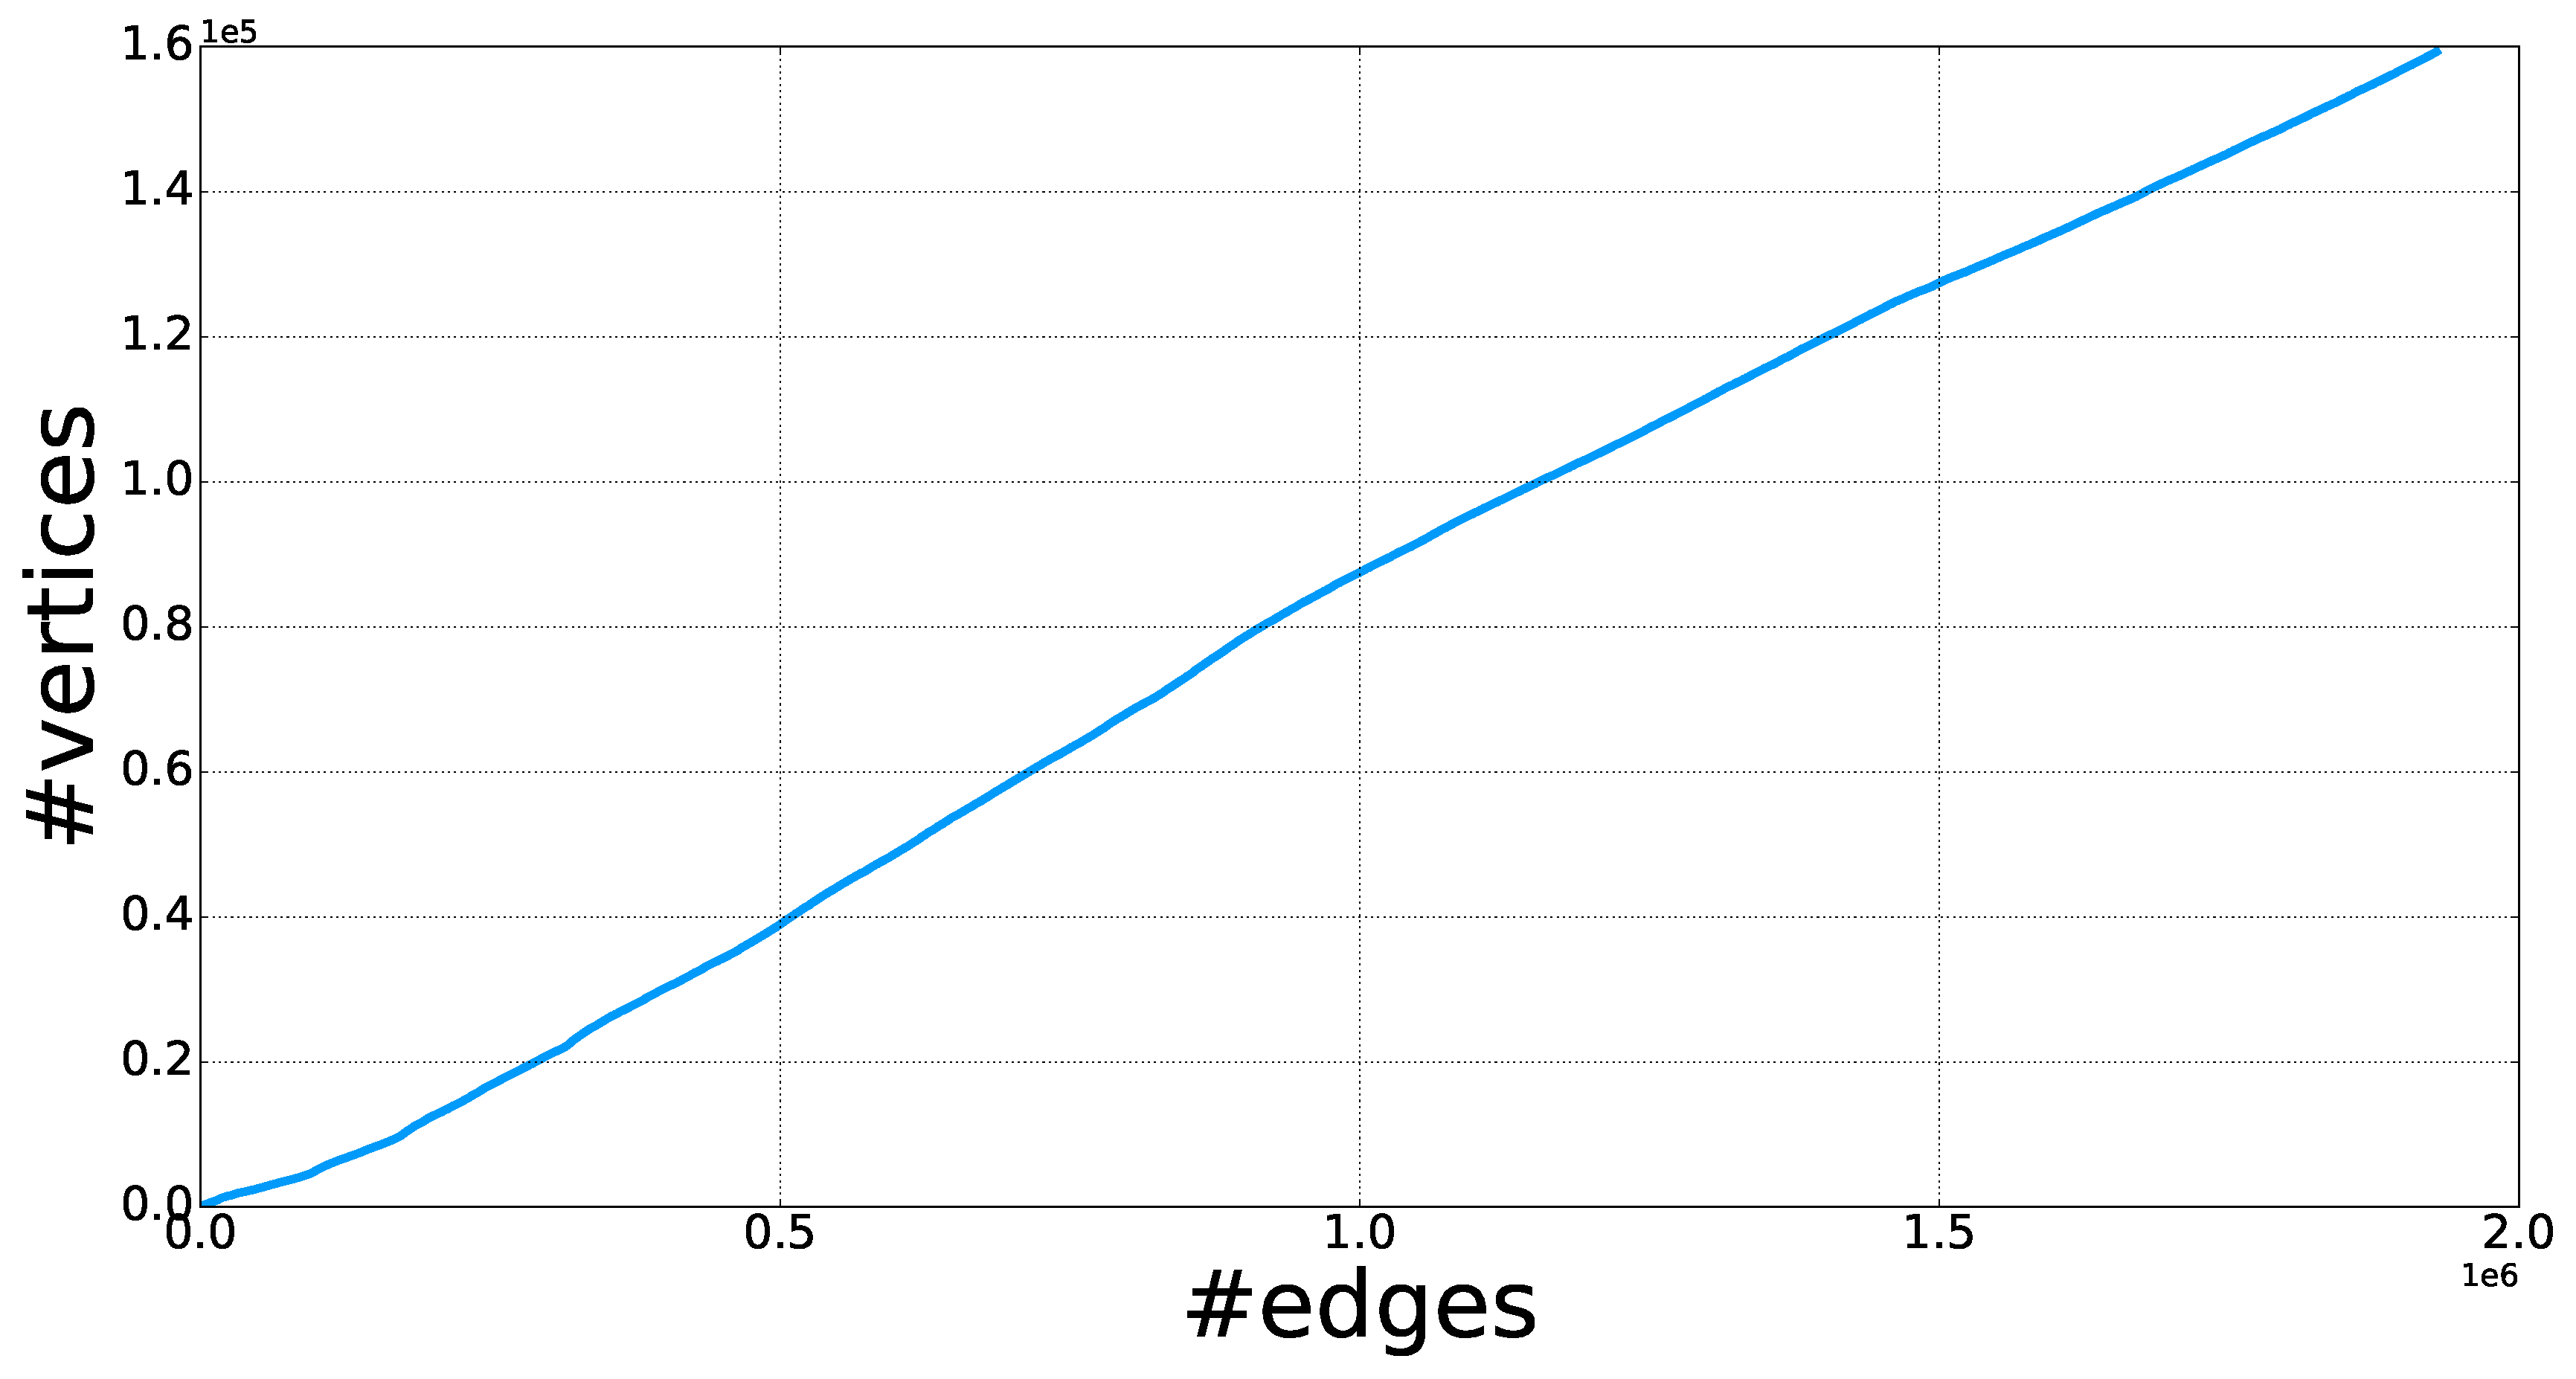
\includegraphics[width=1.0\textwidth]{fig/n_askubuntu_arrival.pdf}
	\end{figure}
	%$\hat{\sigma}=-0.0990787$
	%$\hat{\sigma} = -0.099$
\end{frame}

\begin{frame}
	\frametitle{UCI social network}
	\begin{figure}[h]
		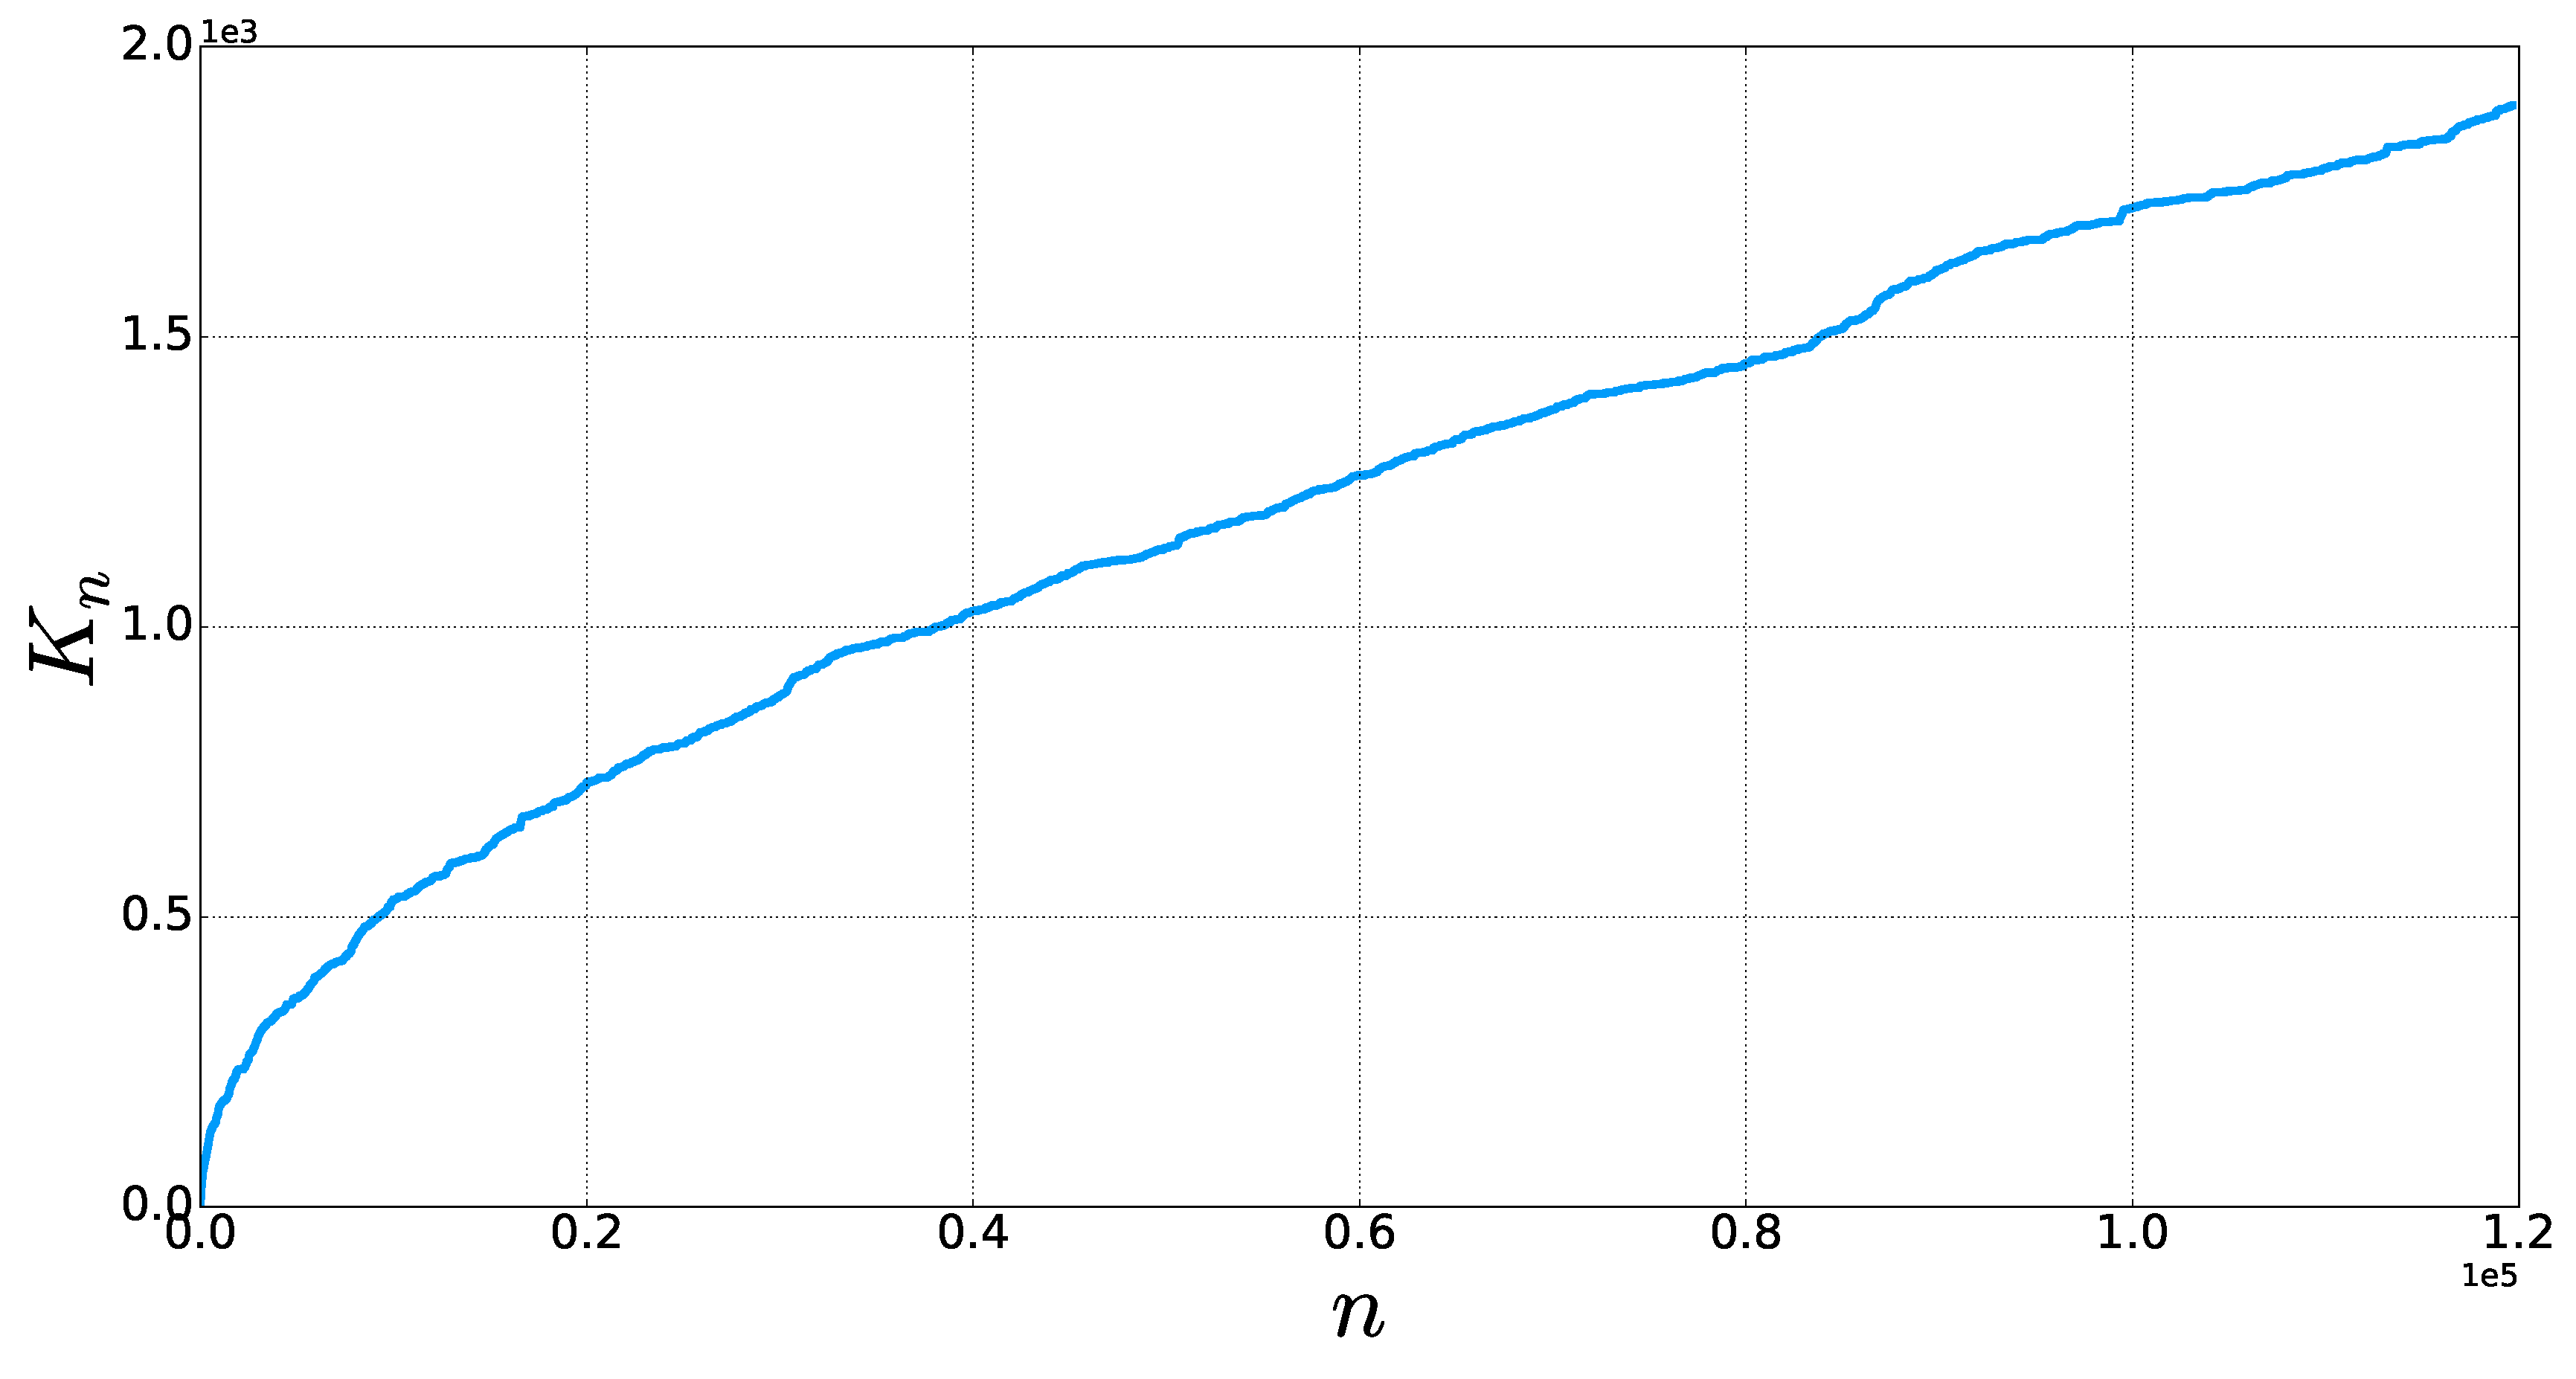
\includegraphics[width=1.0\textwidth]{fig/n_CollegeMsg_arrival.pdf}
	\end{figure}
	% $\sigma=0.95228934$
	% $\hat{\sigma} = 0.952$
\end{frame}

%\begin{frame}
%	\frametitle{Ask Ubuntu degree distribution}
%	\begin{figure}[h]
%		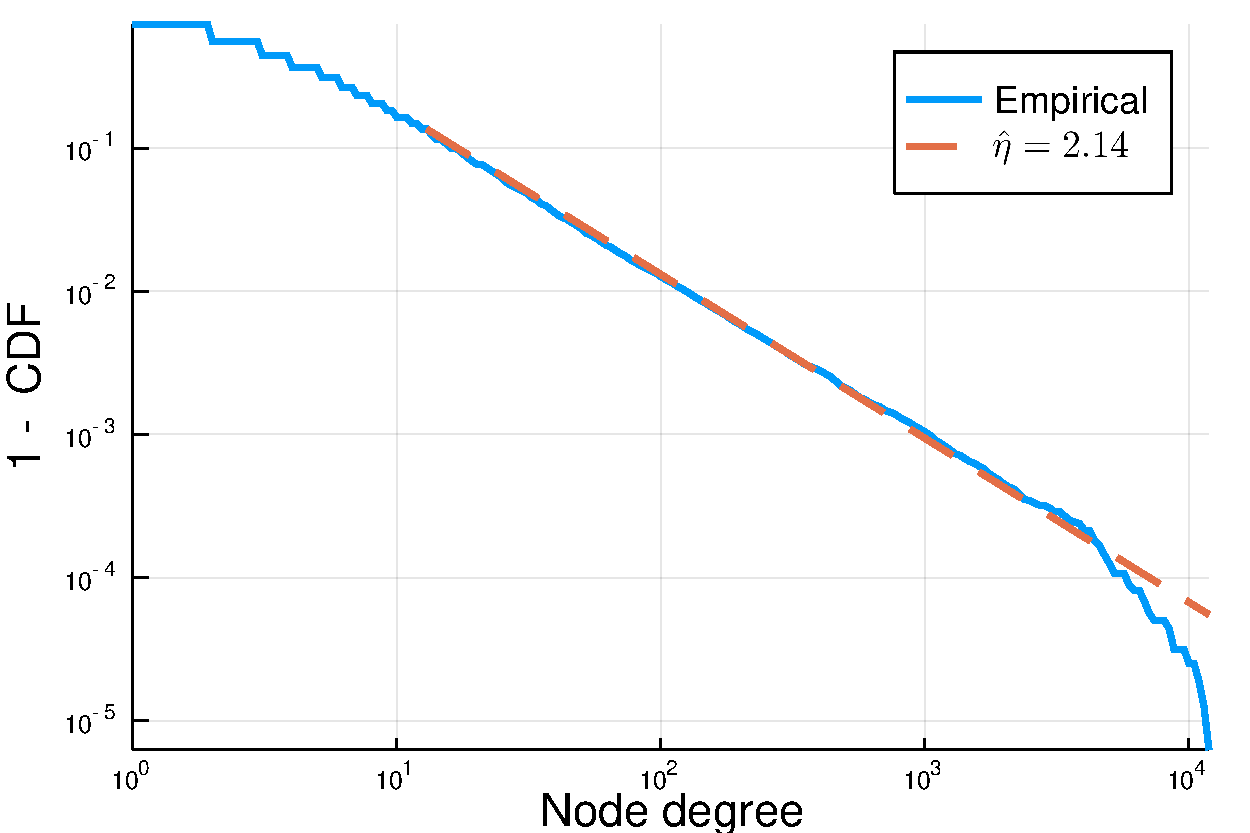
\includegraphics[width=0.8\textwidth]{fig/nodes_degre_power_law_askubuntu.pdf}
%	\end{figure}
%	
%	$\hat{\eta} = 2.14$ estimated using technique of \cite{clauset}
%	
%\end{frame}


\begin{frame}
	\frametitle{Models}
	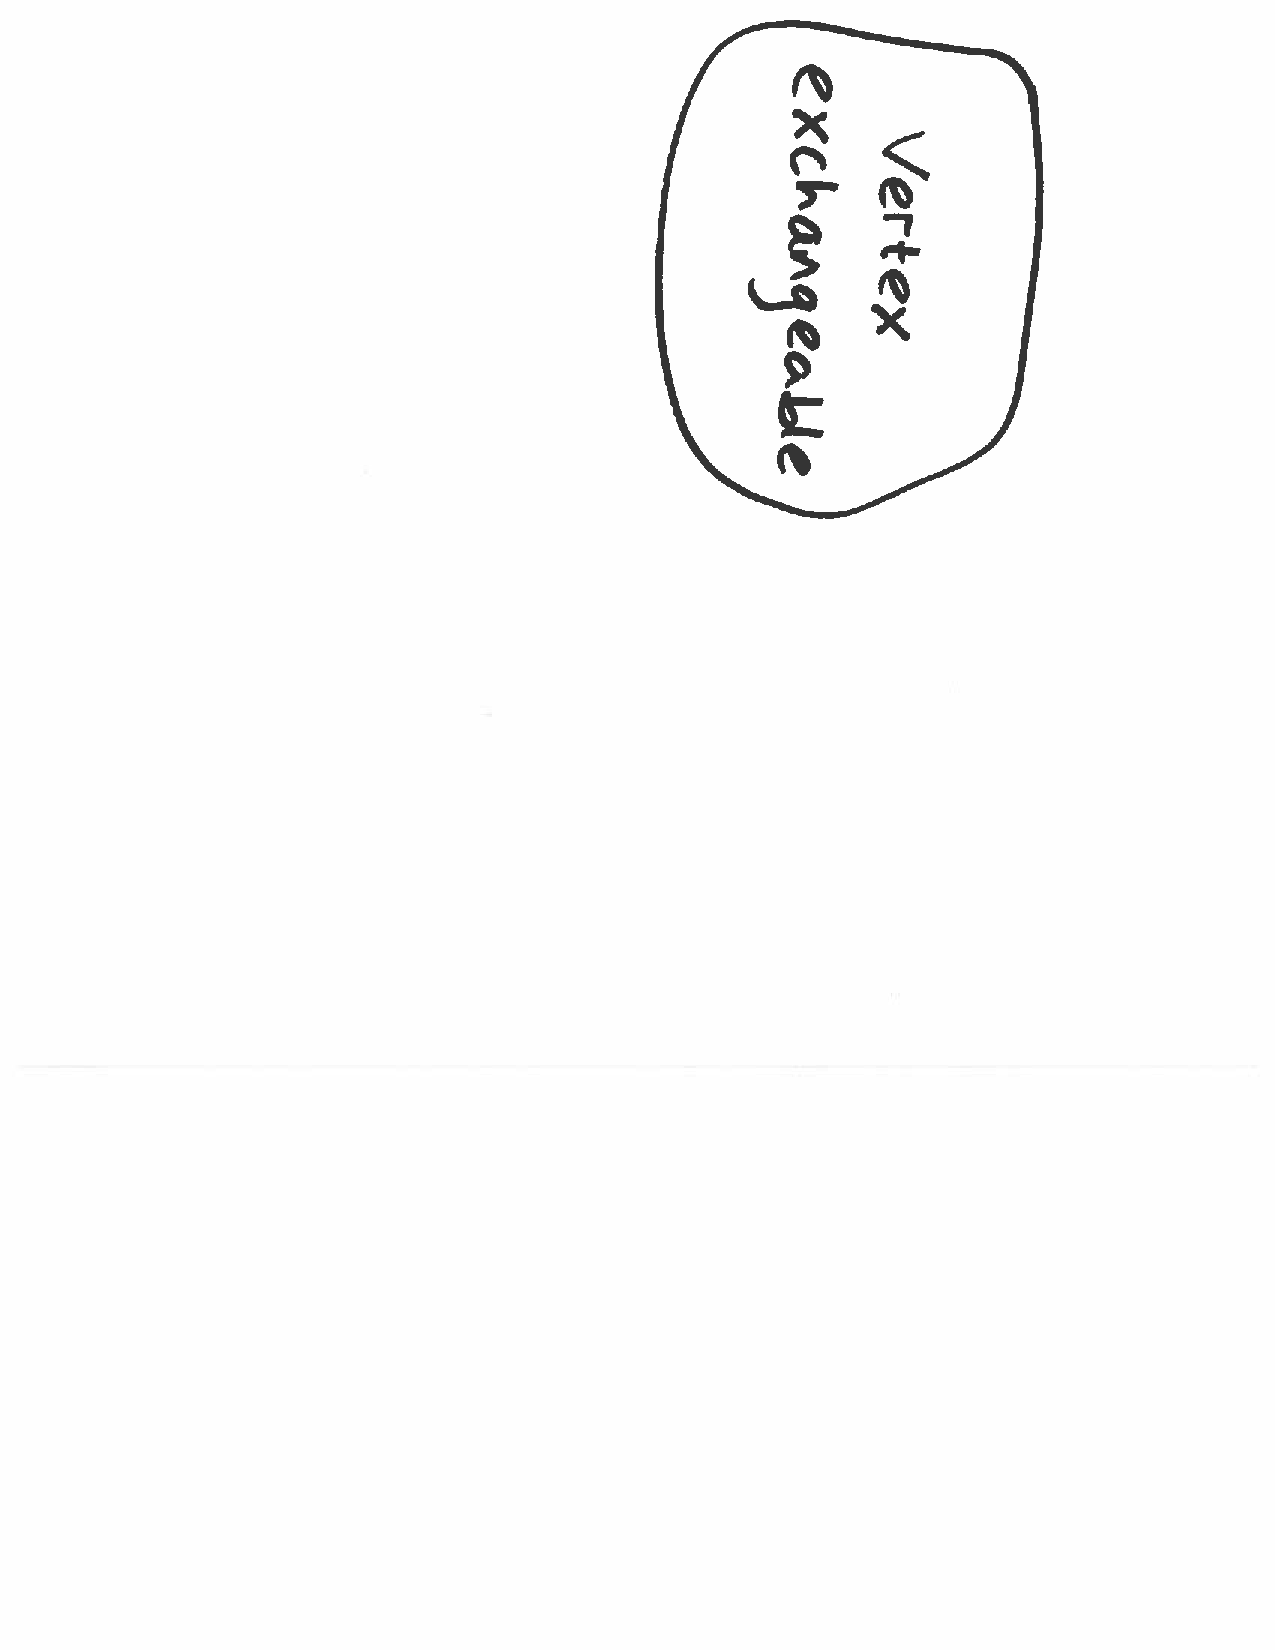
\includegraphics[angle=90,origin=c,scale=0.4]{fig/models1}
\end{frame}

\begin{frame}
	\frametitle{Models}
	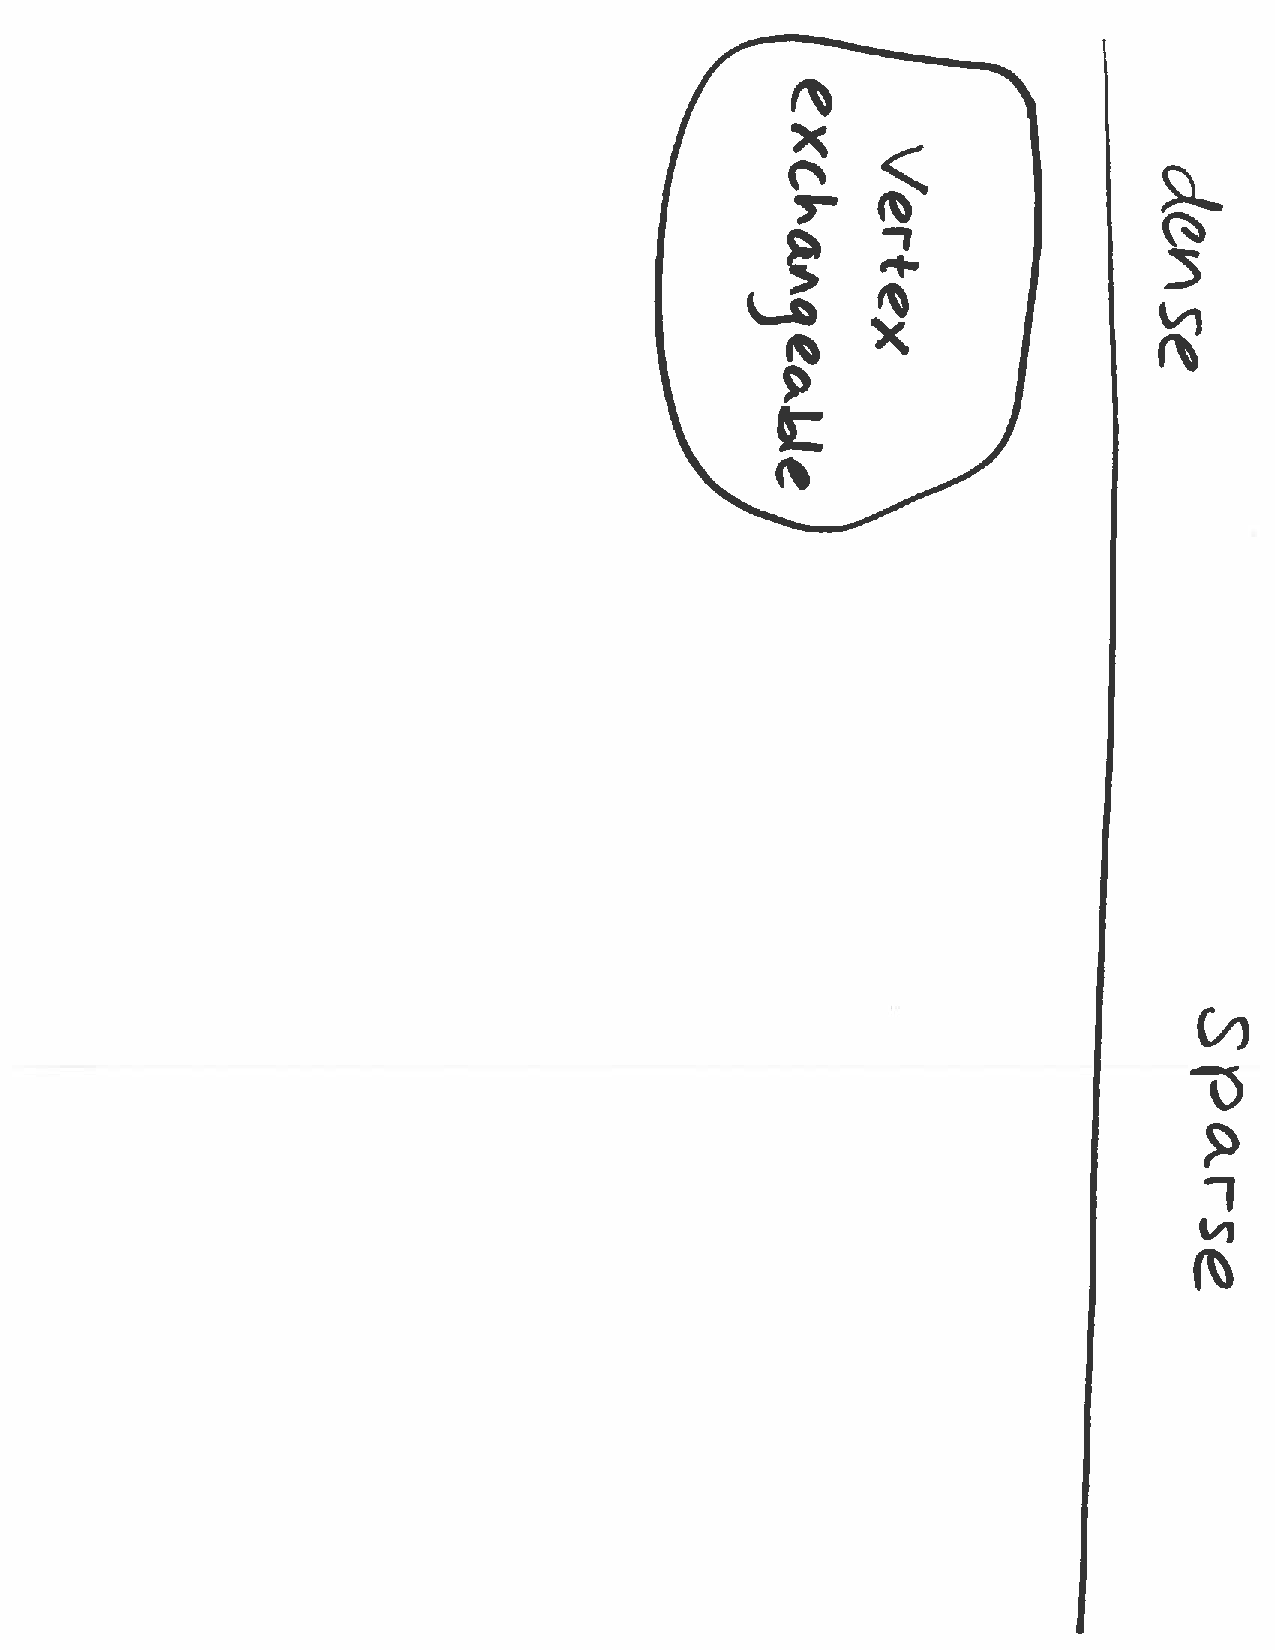
\includegraphics[angle=90,origin=c,scale=0.4]{fig/models2}
\end{frame}

\begin{frame}
	\frametitle{Models}
	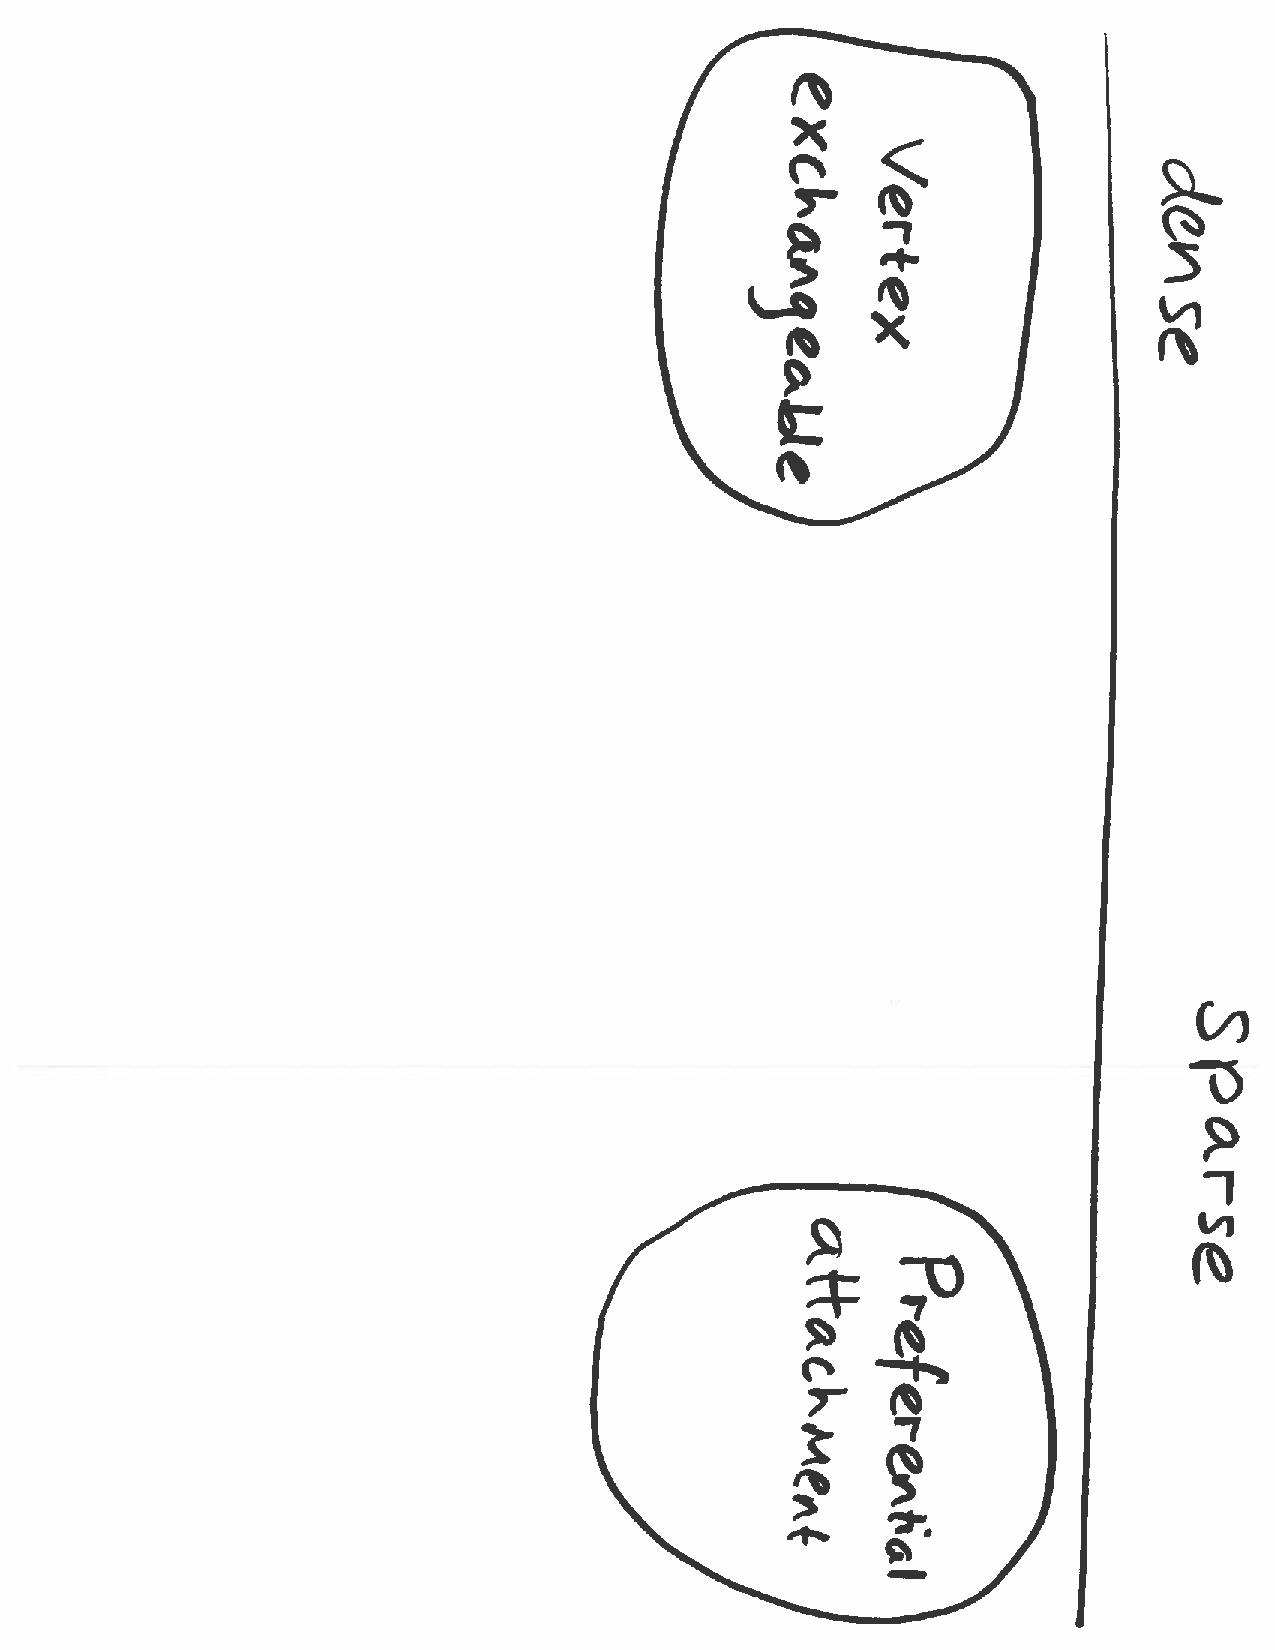
\includegraphics[angle=90,origin=c,scale=0.4]{fig/models3}
\end{frame}

\begin{frame}
	\frametitle{Models}
	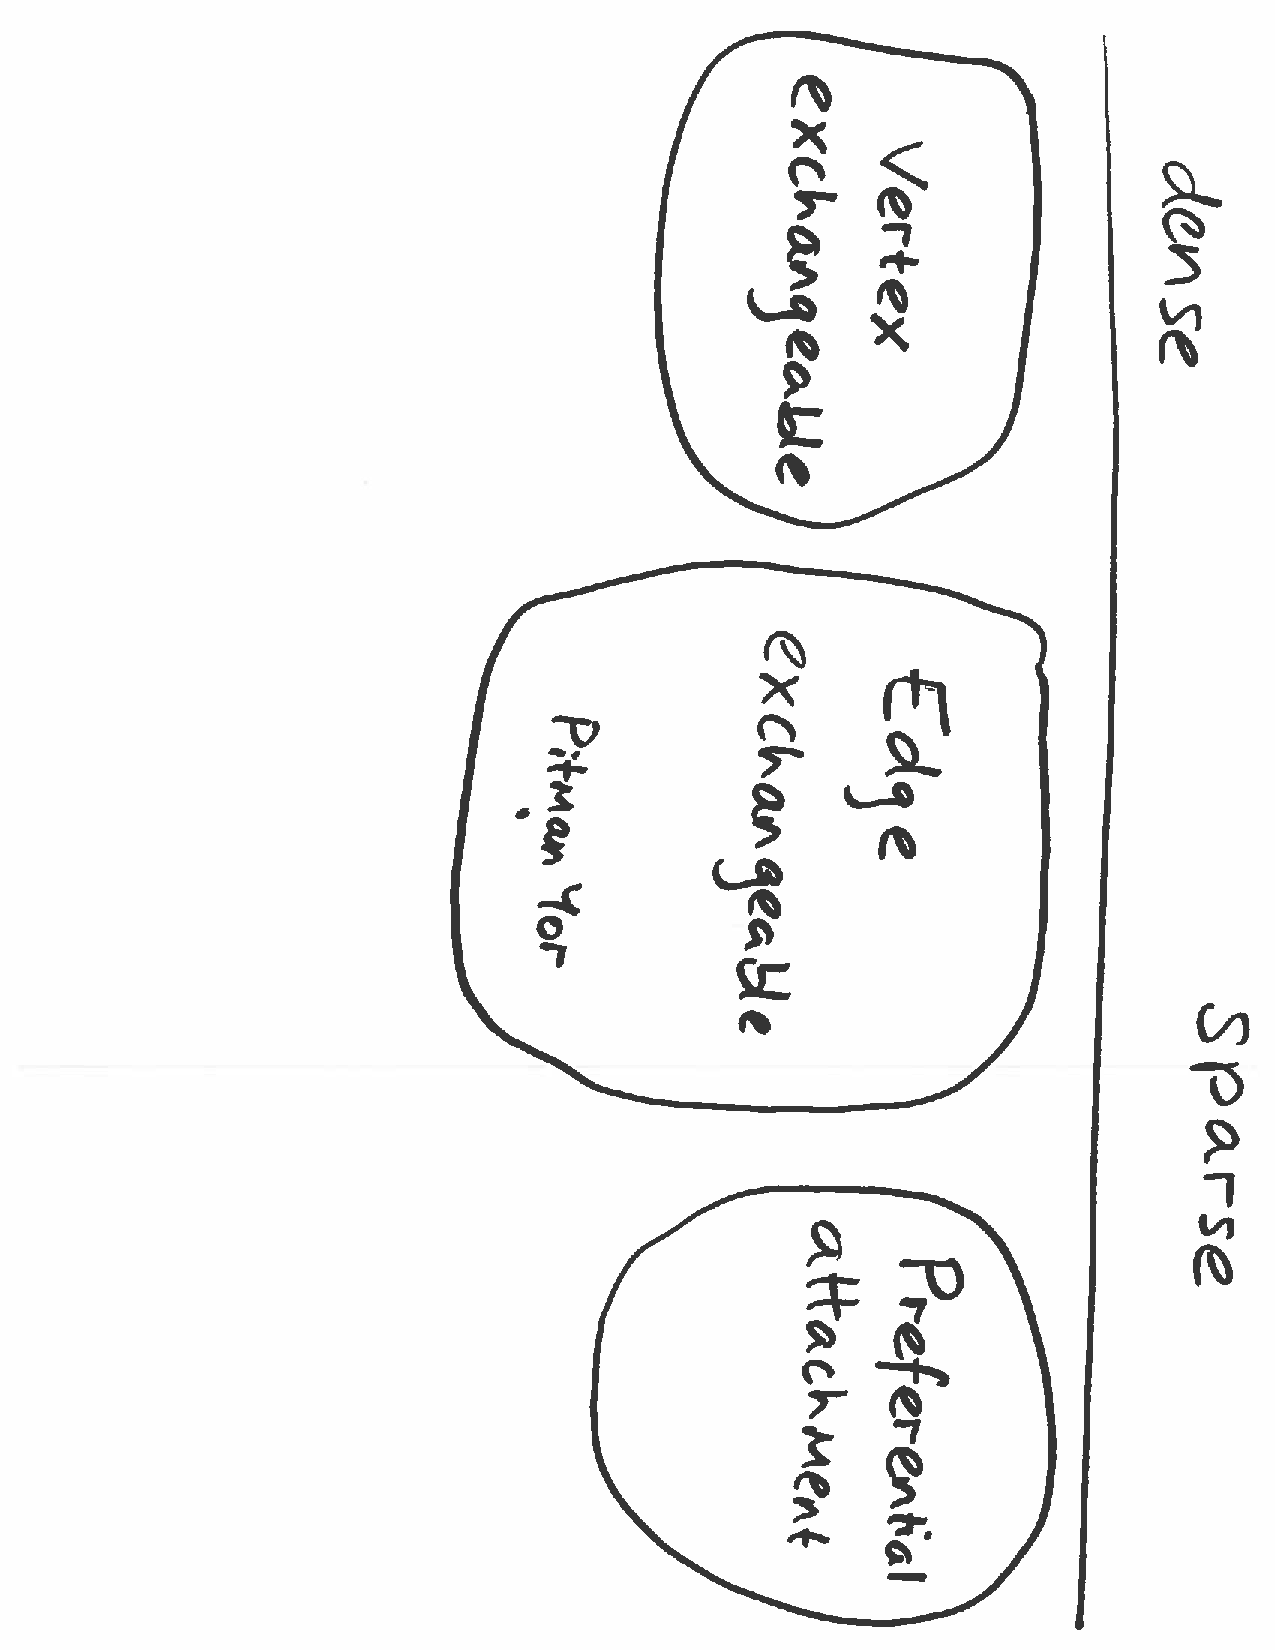
\includegraphics[angle=90,origin=c,scale=0.4]{fig/models4}
\end{frame}

\begin{frame}
	\frametitle{Edge exchangeable models \cite{cai2016}, \cite{CraneDempsey2017}}
	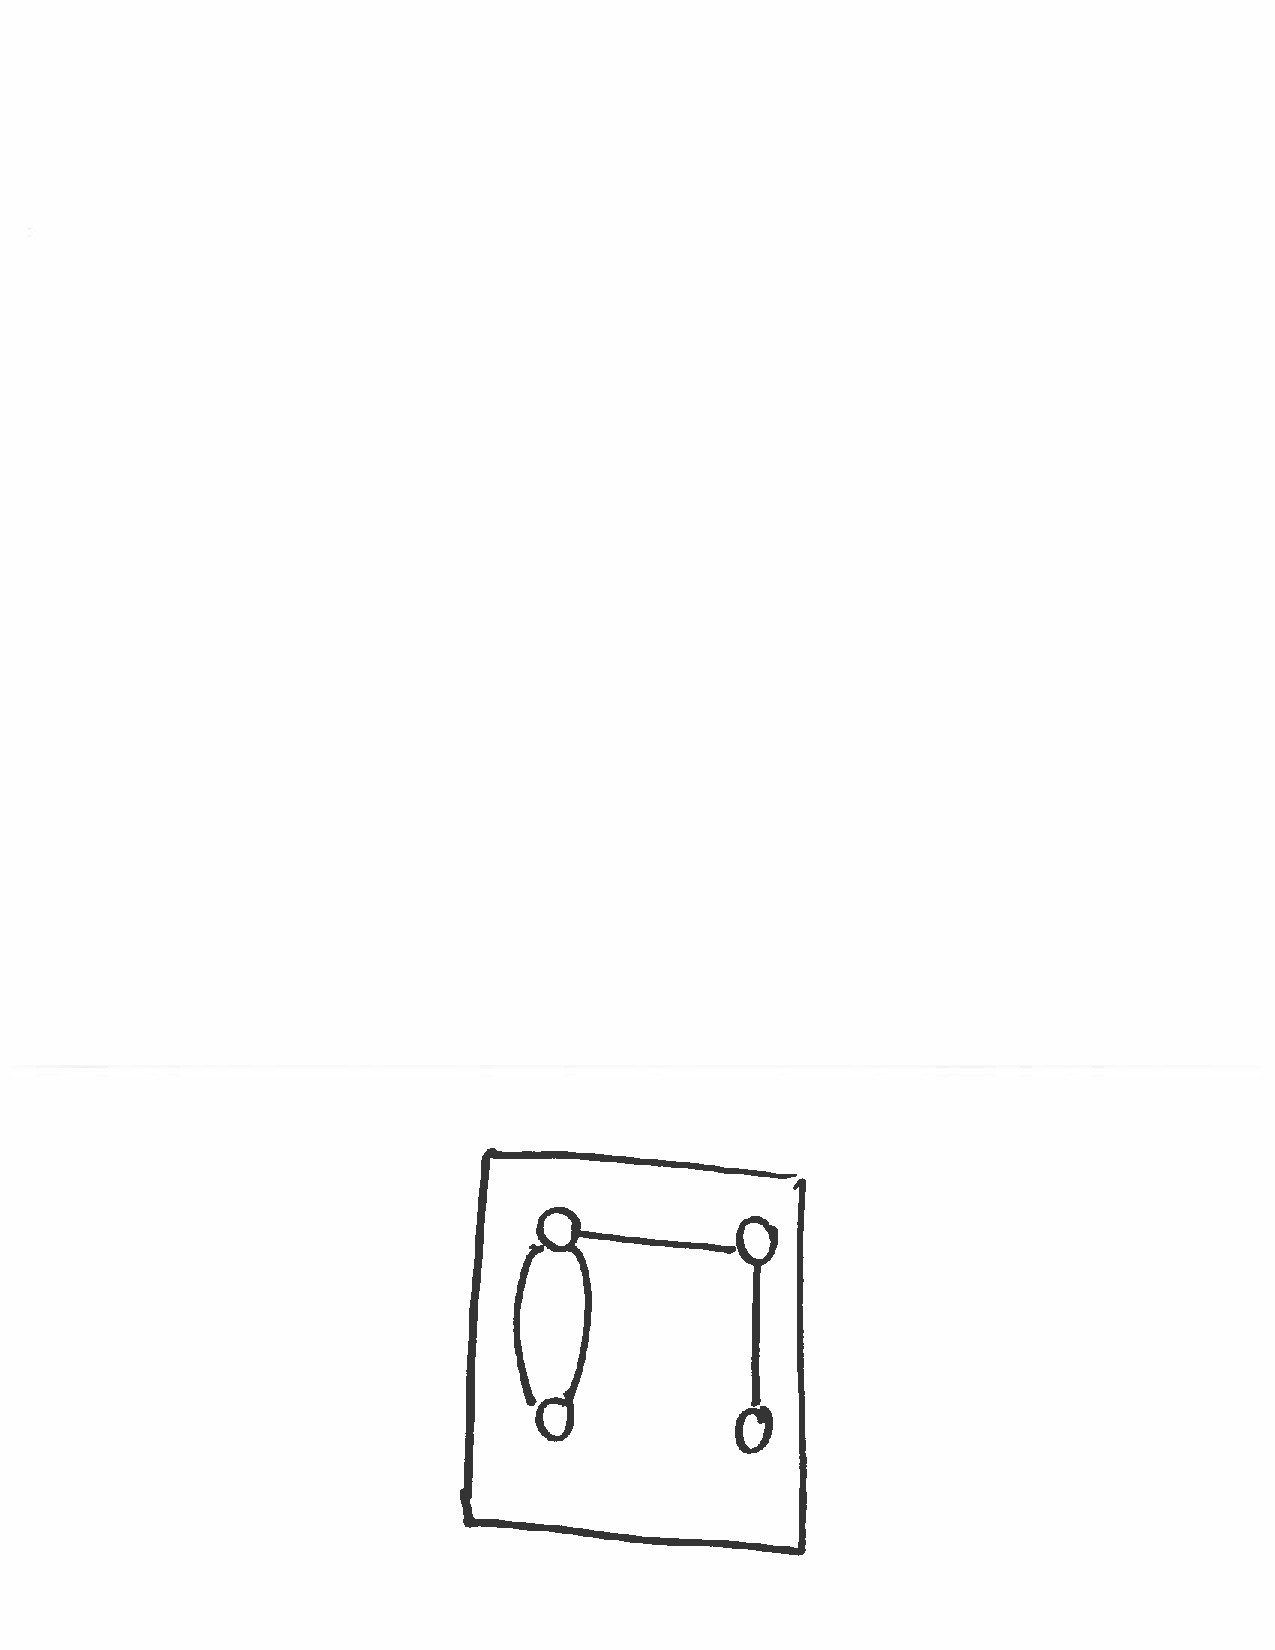
\includegraphics[angle=90,origin=c,scale=0.4]{fig/ee1}
\end{frame}

\begin{frame}
	\frametitle{Edge exchangeable models \cite{cai2016}, \cite{CraneDempsey2017}}
	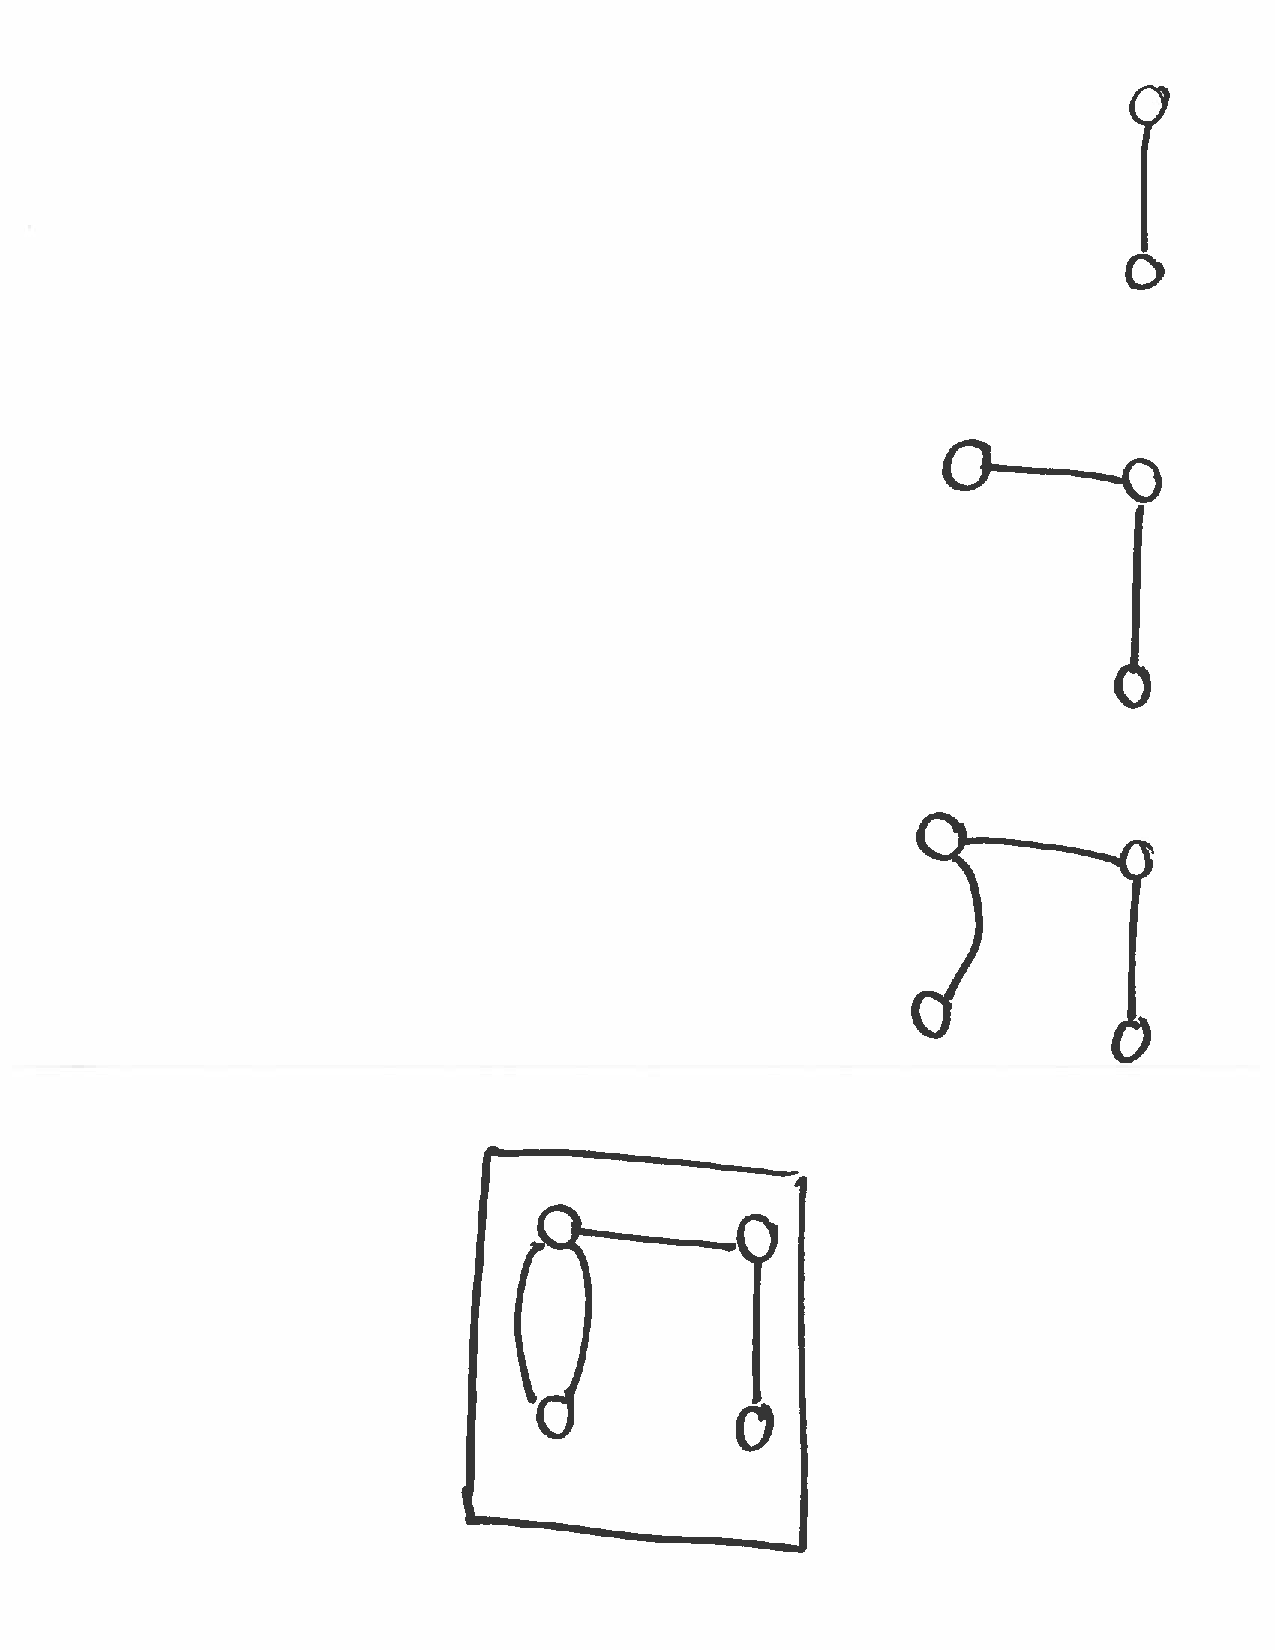
\includegraphics[angle=90,origin=c,scale=0.4]{fig/ee2}
\end{frame}

\begin{frame}
	\frametitle{Edge exchangeable models \cite{cai2016}, \cite{CraneDempsey2017}}
	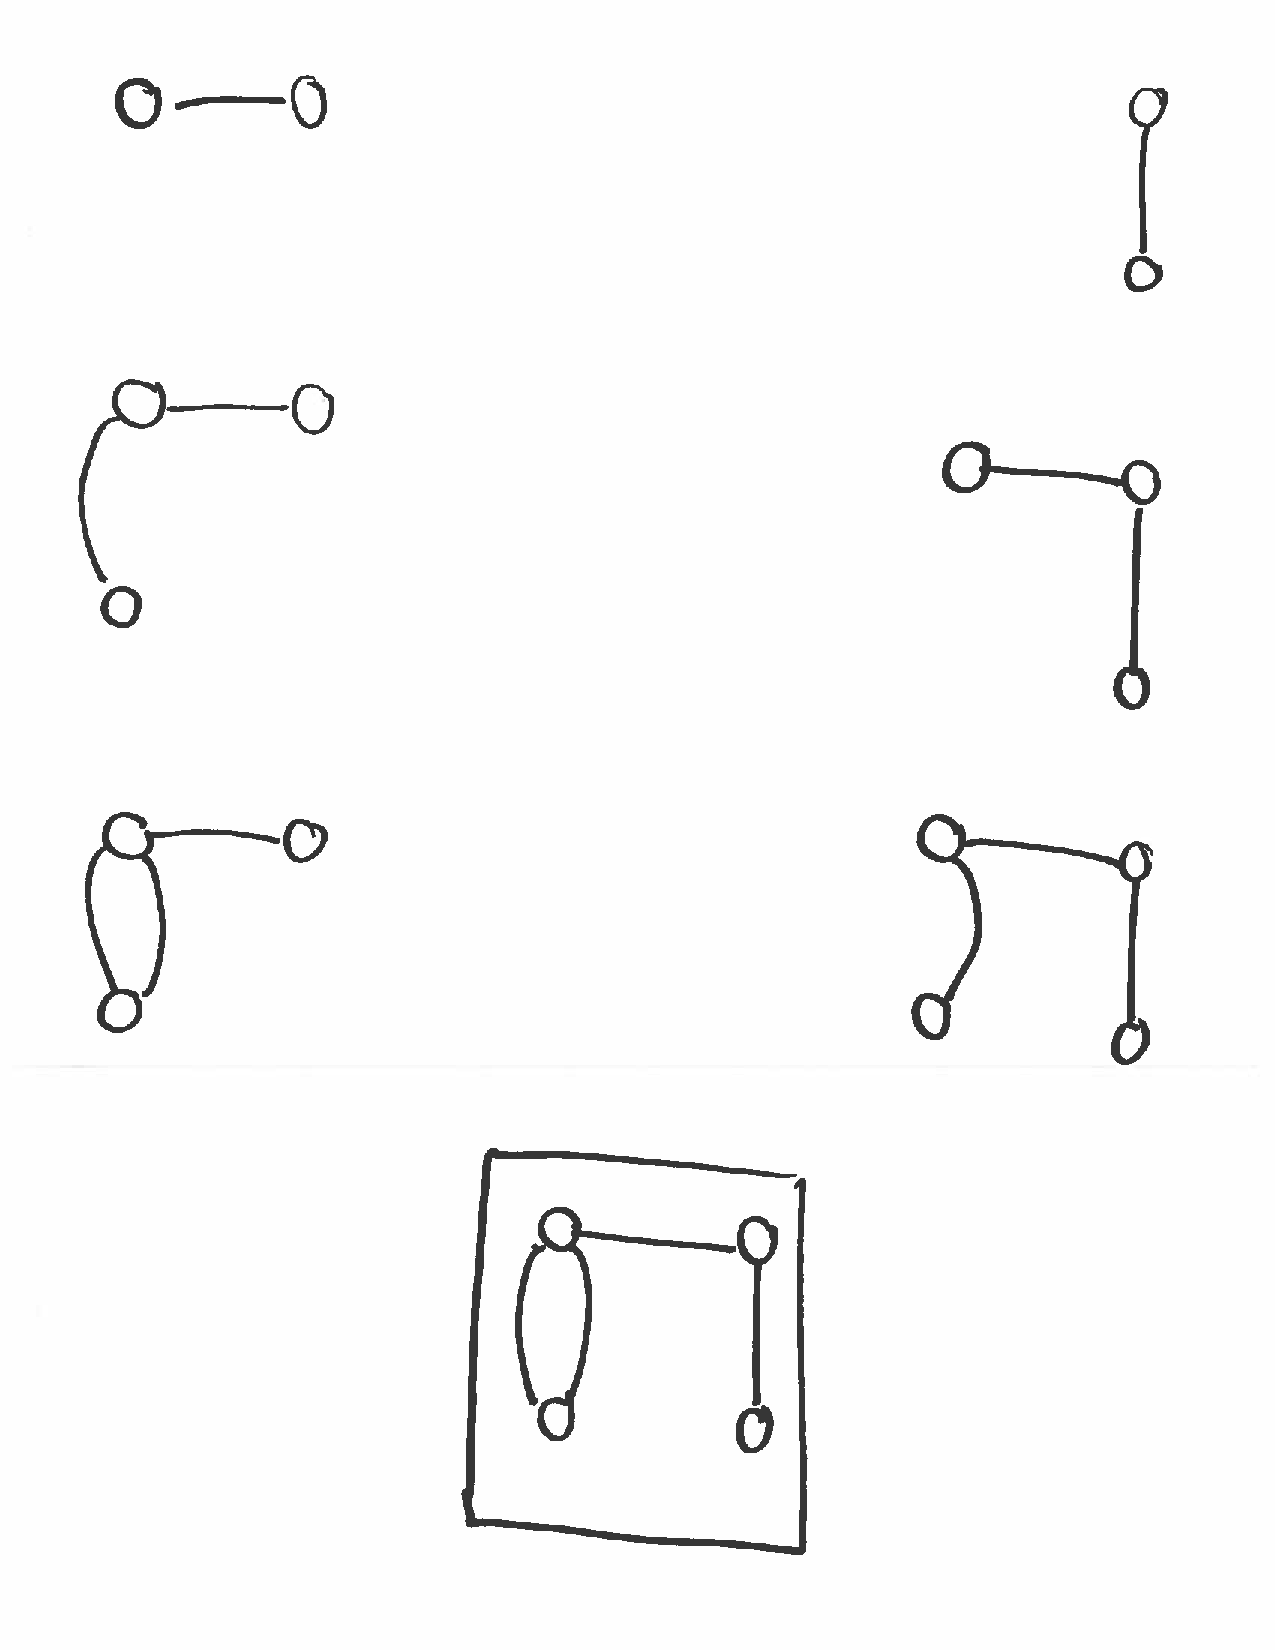
\includegraphics[angle=90,origin=c,scale=0.4]{fig/ee3}
\end{frame}

\begin{frame}
	\frametitle{Paintbox representation}
	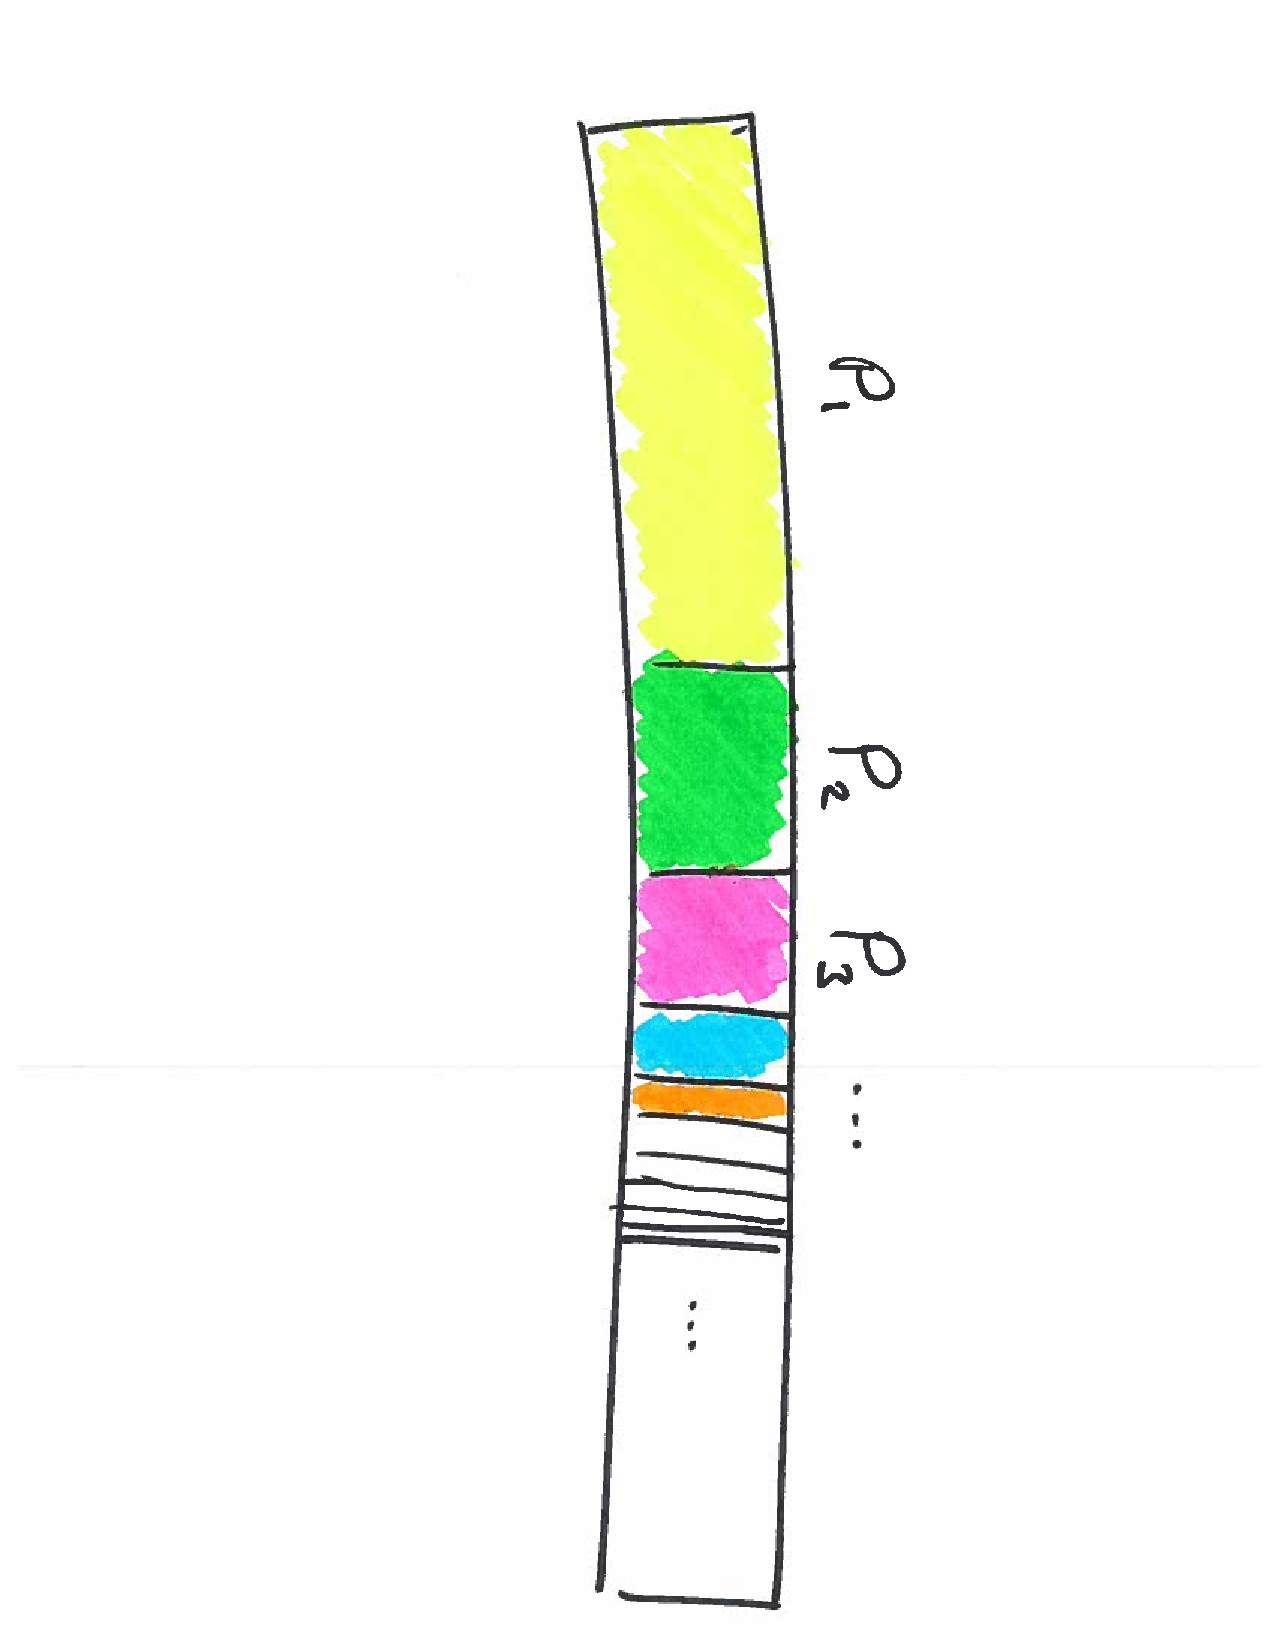
\includegraphics[angle=90,origin=c,scale=0.4]{fig/paintbox}
\end{frame}

\begin{frame}
	\frametitle{Paintbox representation}
	Consequence\begin{itemize}
		\item Edge exchangeable models have sublinear sparsity
	\end{itemize}
\end{frame}

\begin{frame}
	\frametitle{Models}
	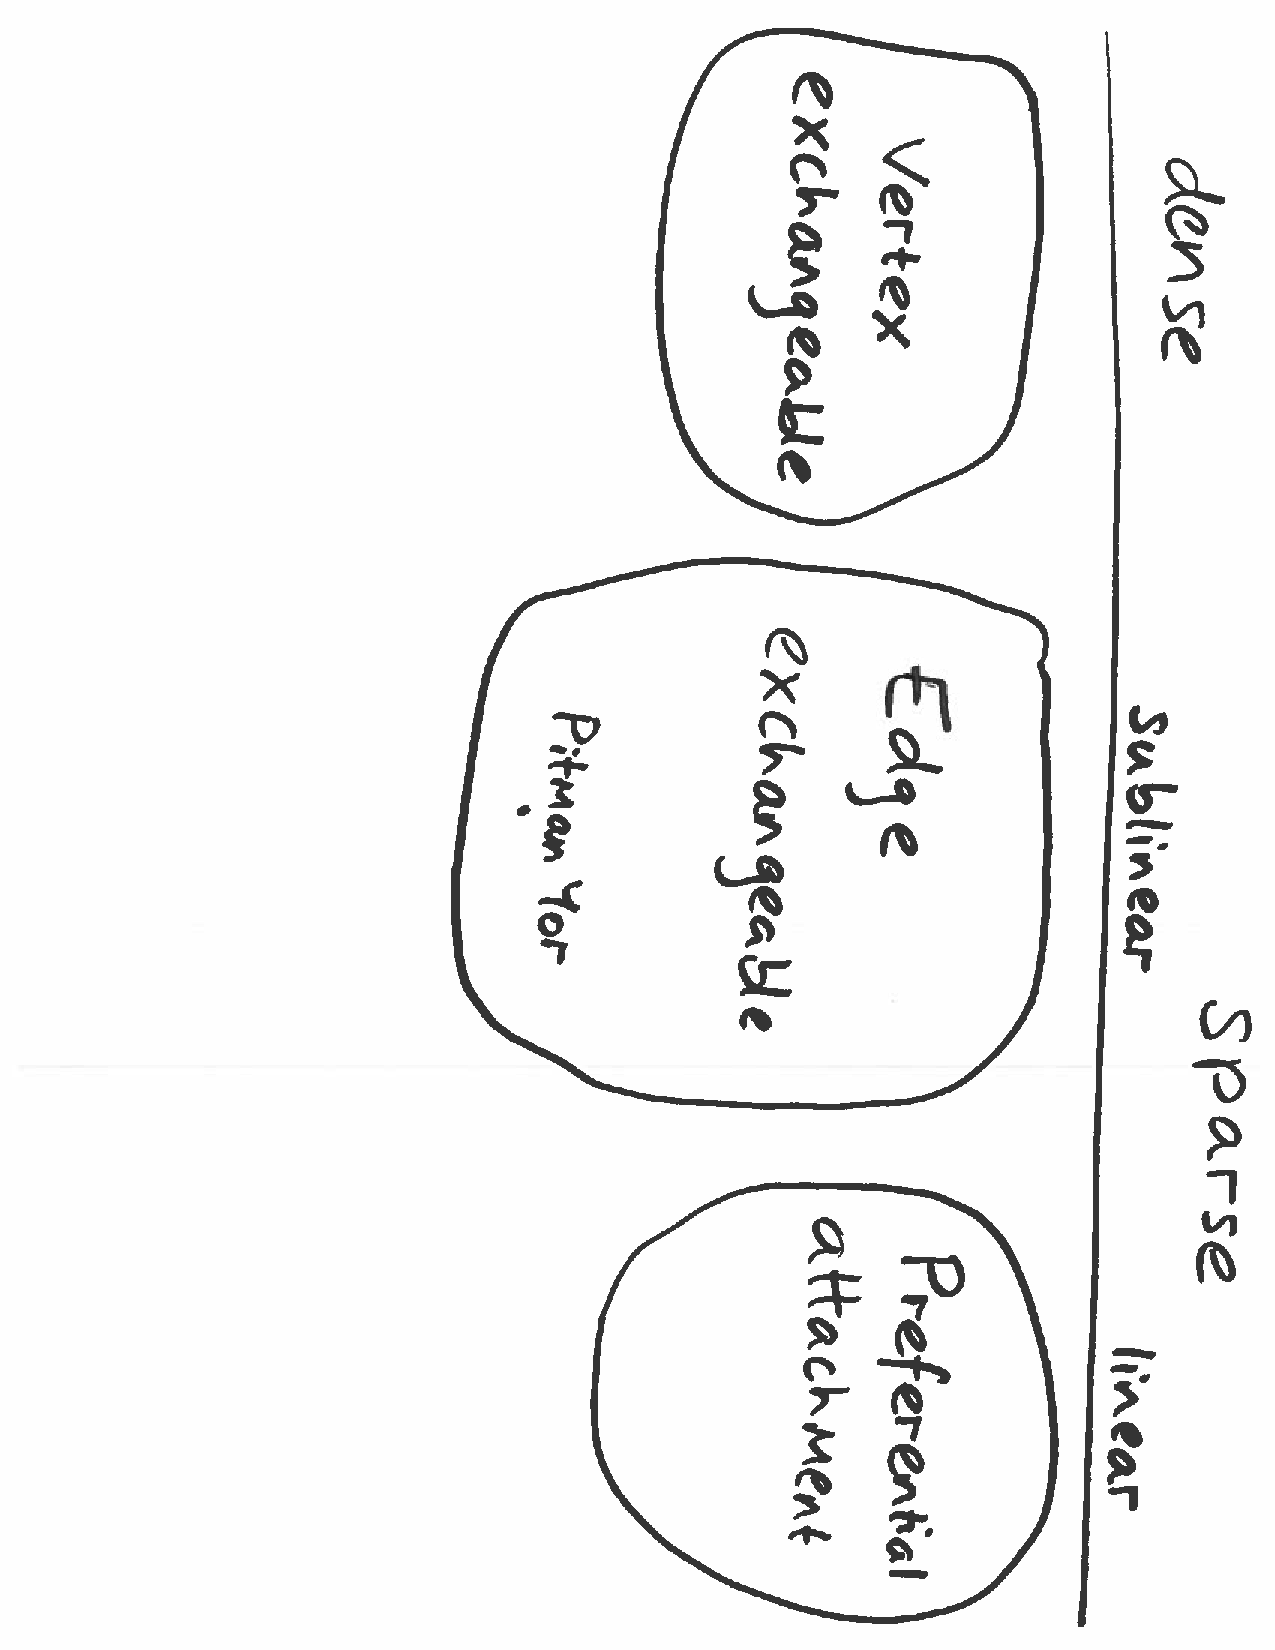
\includegraphics[angle=90,origin=c,scale=0.4]{fig/models5}
\end{frame}

\begin{frame}
	\frametitle{Models}
	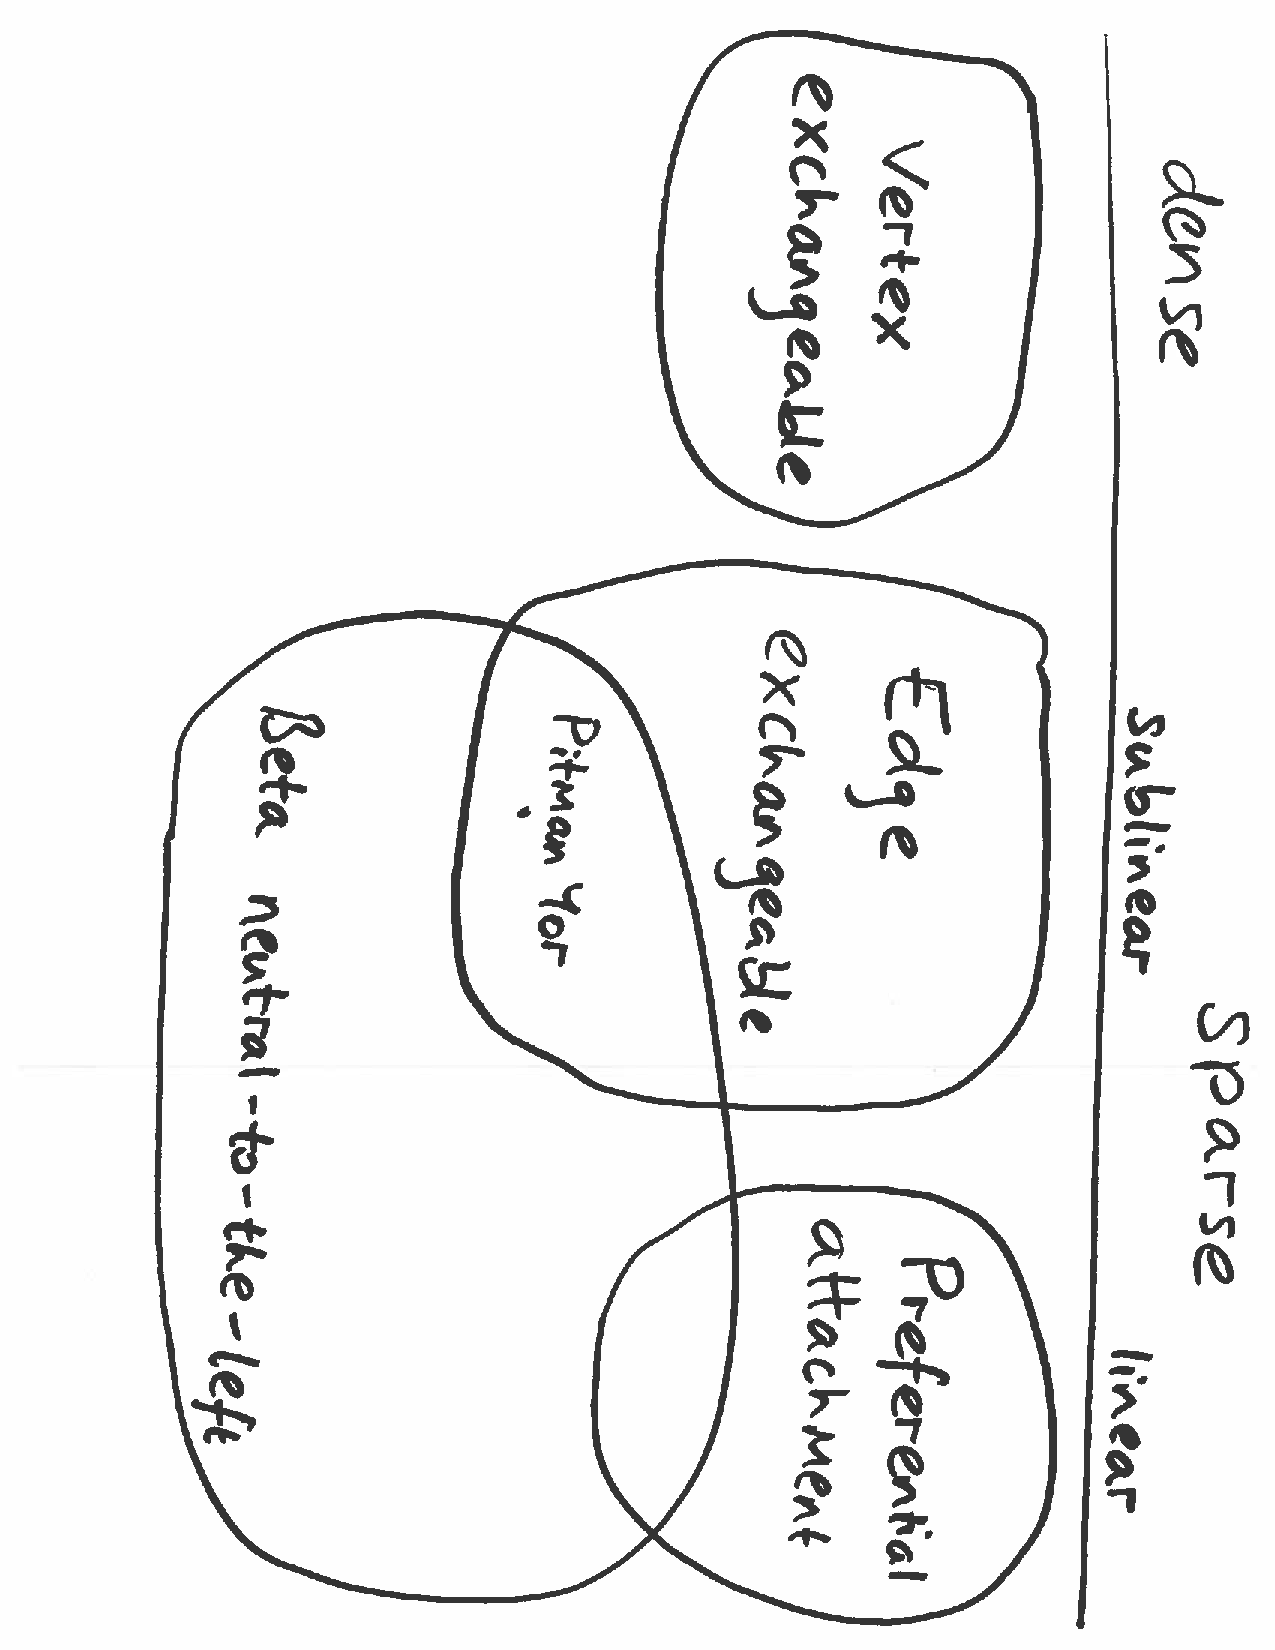
\includegraphics[angle=90,origin=c,scale=0.4]{fig/models6}
\end{frame}

\begin{frame}
	\frametitle{Models}
	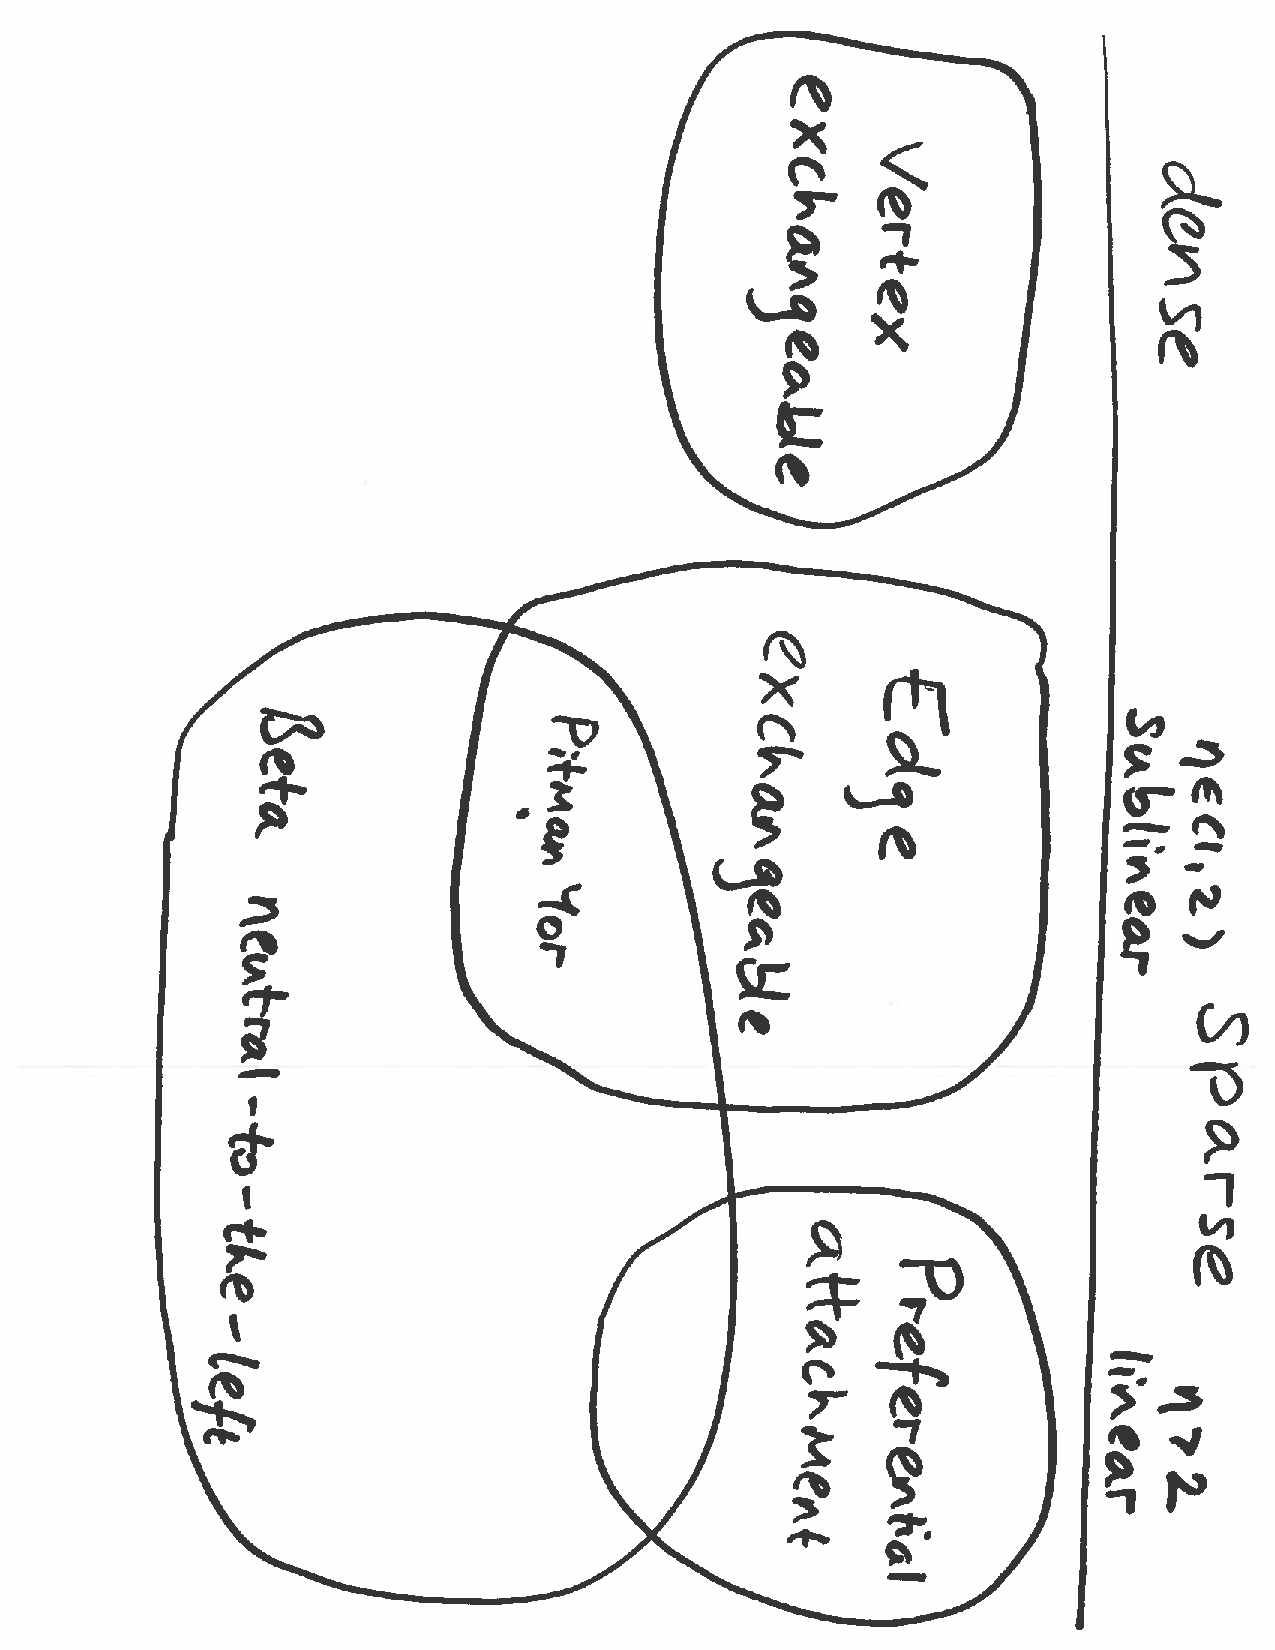
\includegraphics[angle=90,origin=c,scale=0.4]{fig/models7}
\end{frame}

\begin{frame}
	\frametitle{Beta Neutral-to-the-left Model \cite{Bloem2017}}
	\vspace{2pt}
	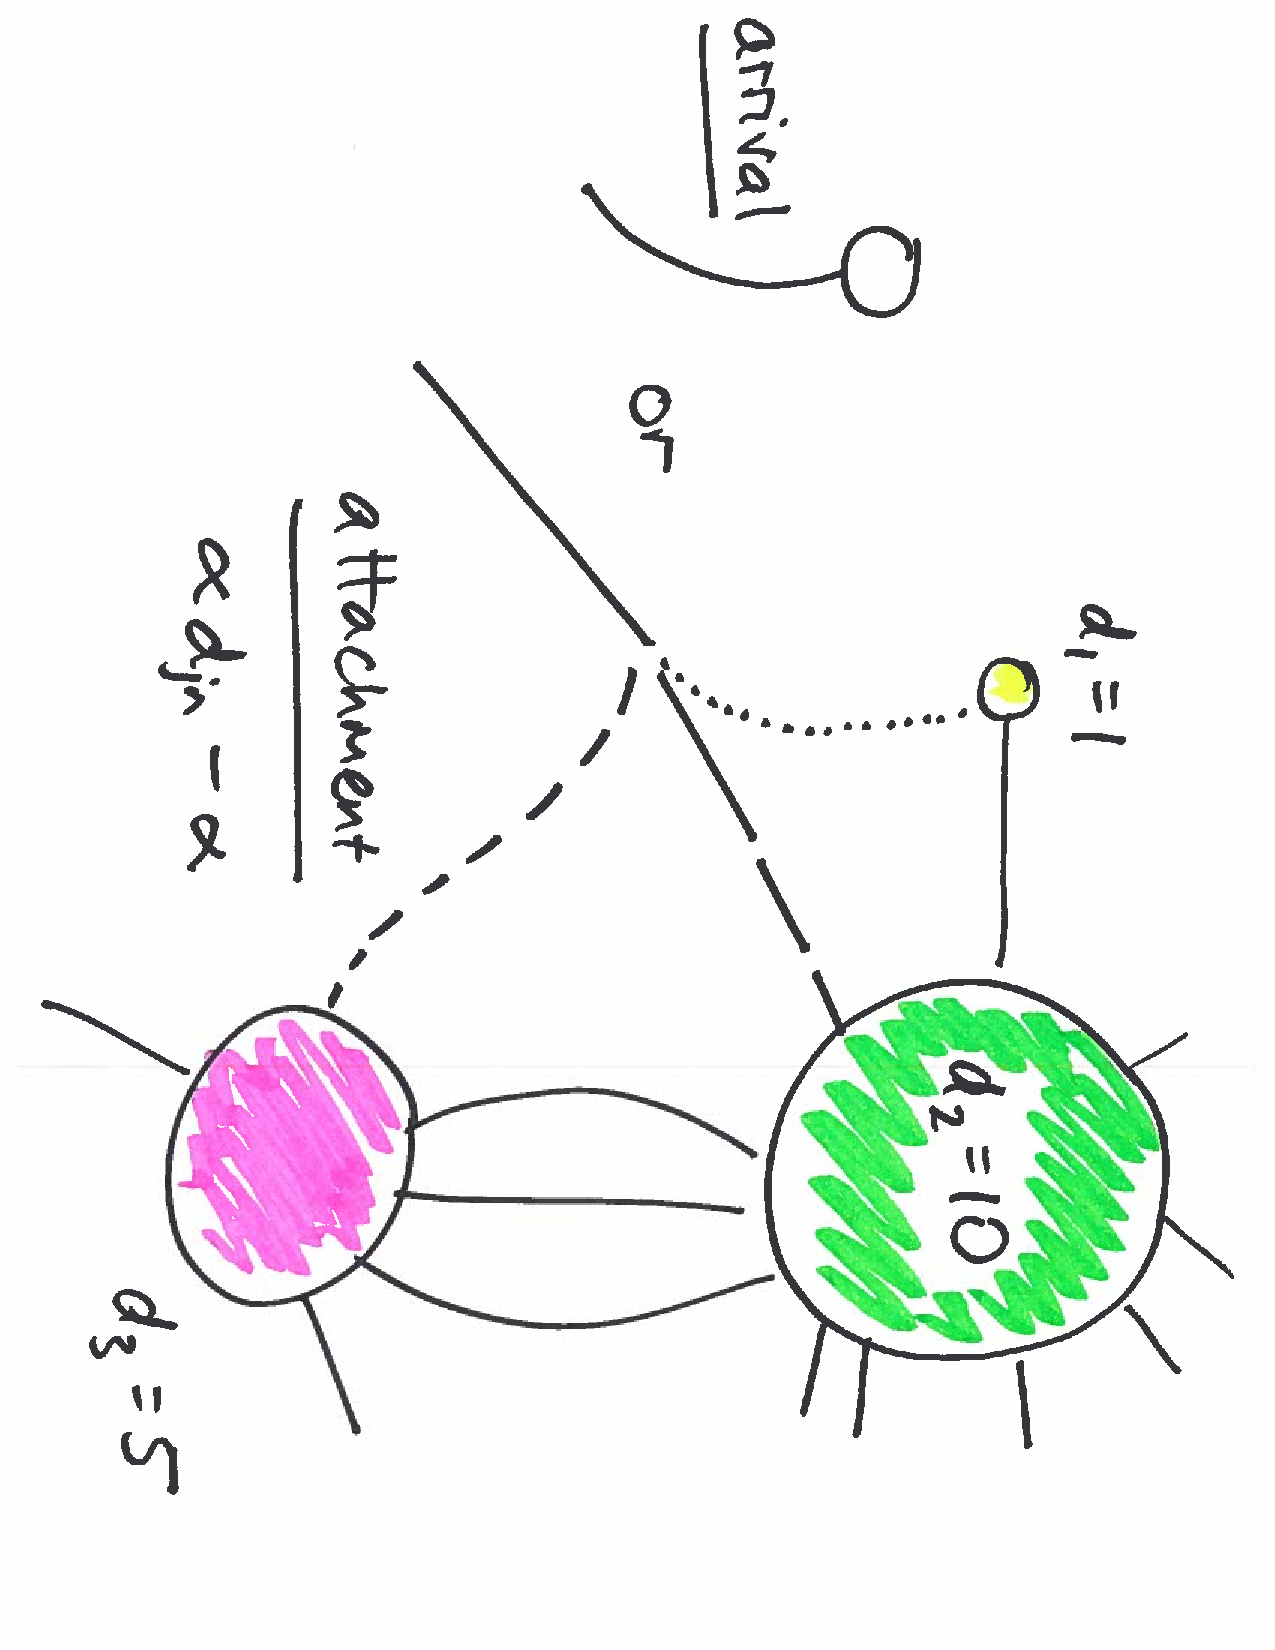
\includegraphics[angle=90,origin=c,scale=0.37]{fig/bntl}
\end{frame}

%\begin{frame}
%	\frametitle{Hierarchical representation of BNTL process}
%	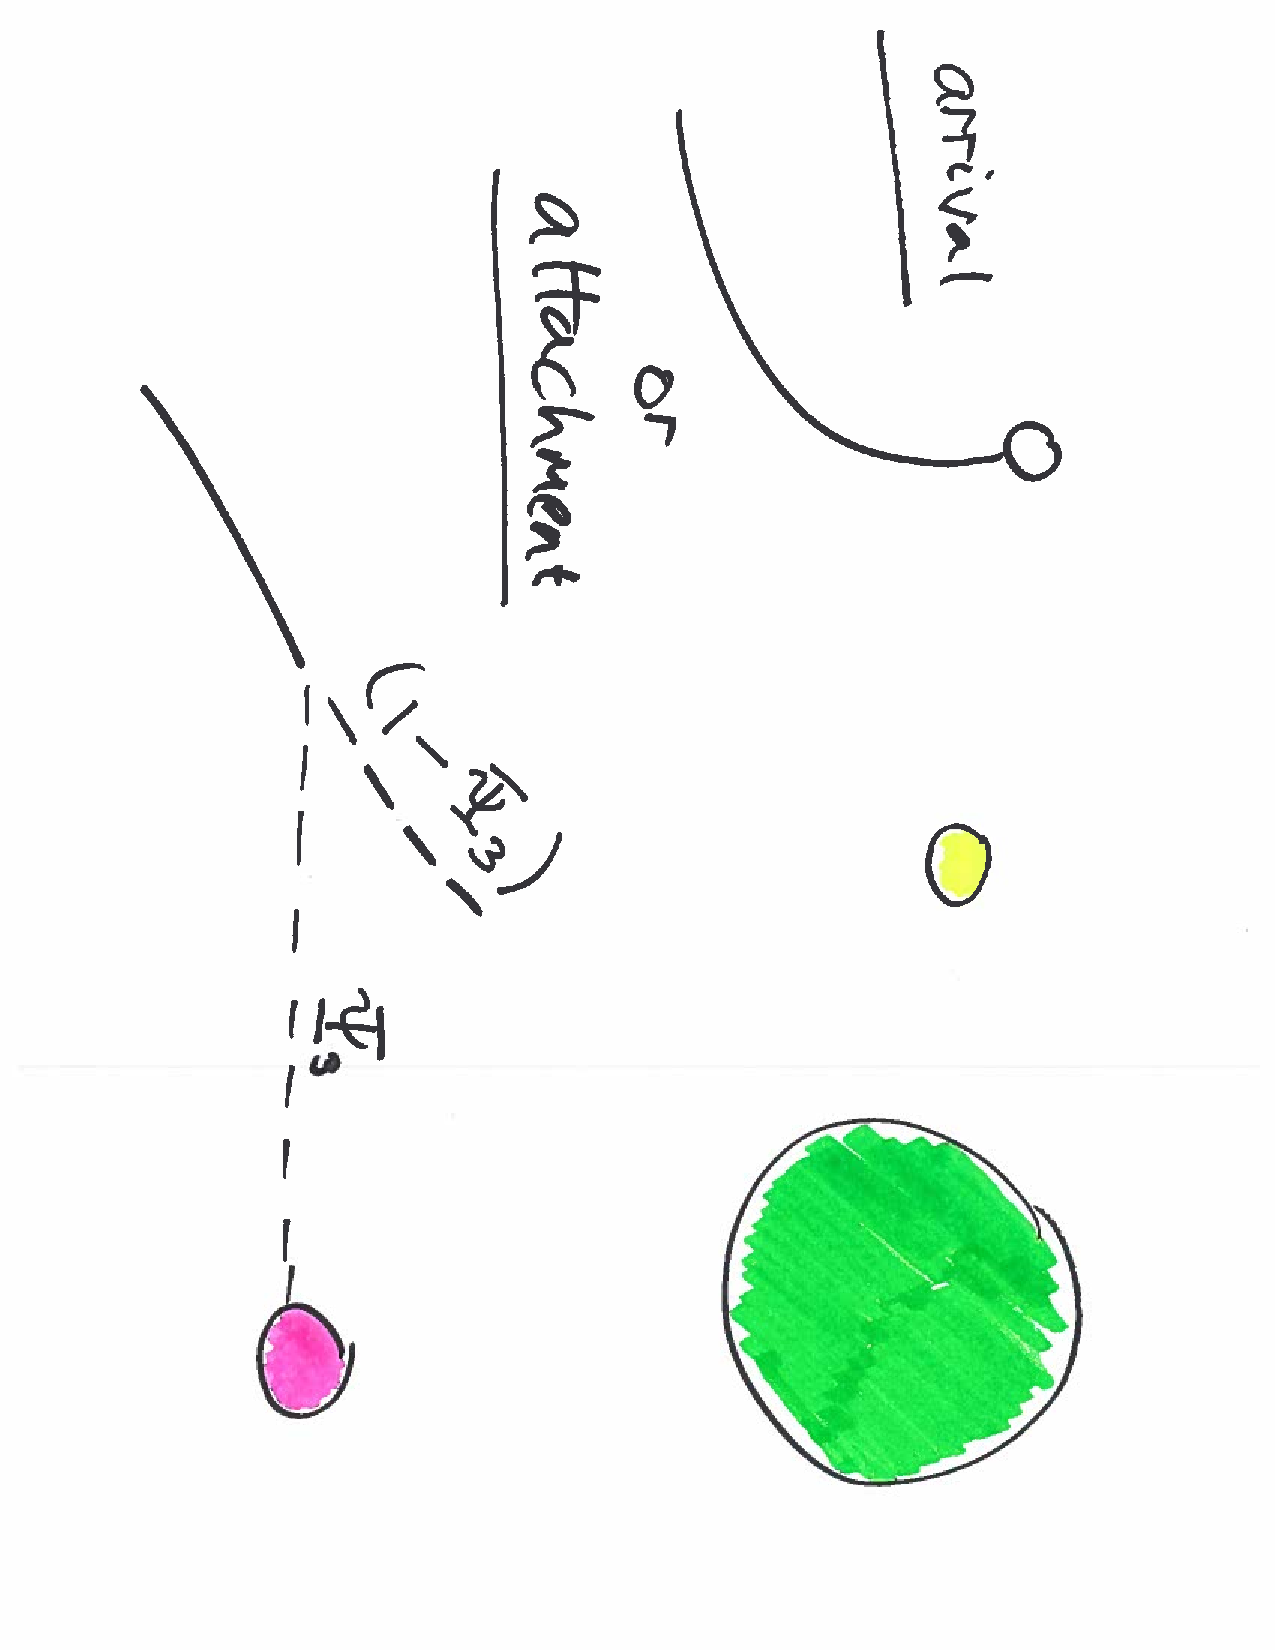
\includegraphics[angle=90,origin=c,scale=0.4]{fig/bntllatent1}
%\end{frame}
%
%\begin{frame}
%	\frametitle{Hierarchical representation of BNTL process}
%	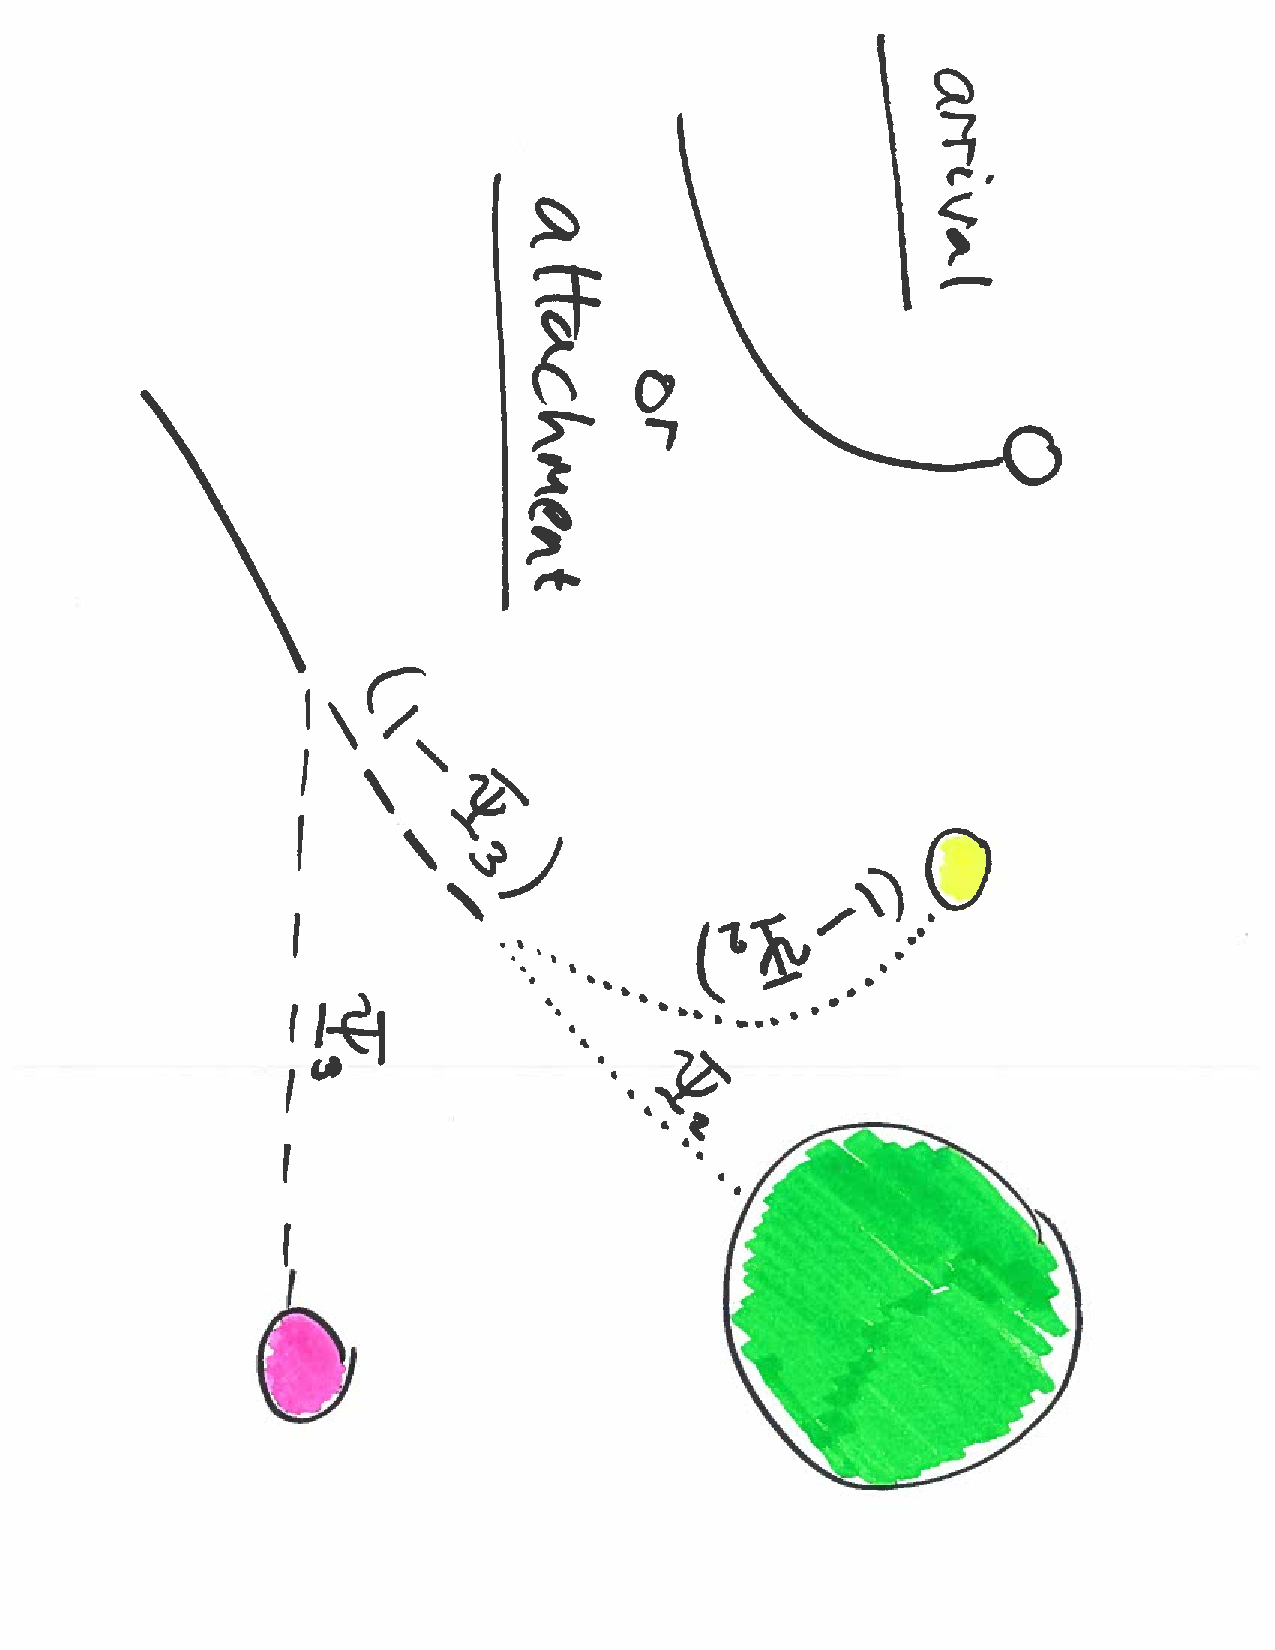
\includegraphics[angle=90,origin=c,scale=0.4]{fig/bntllatent2}
%\end{frame}

\begin{frame}
	\frametitle{Latent representation}
	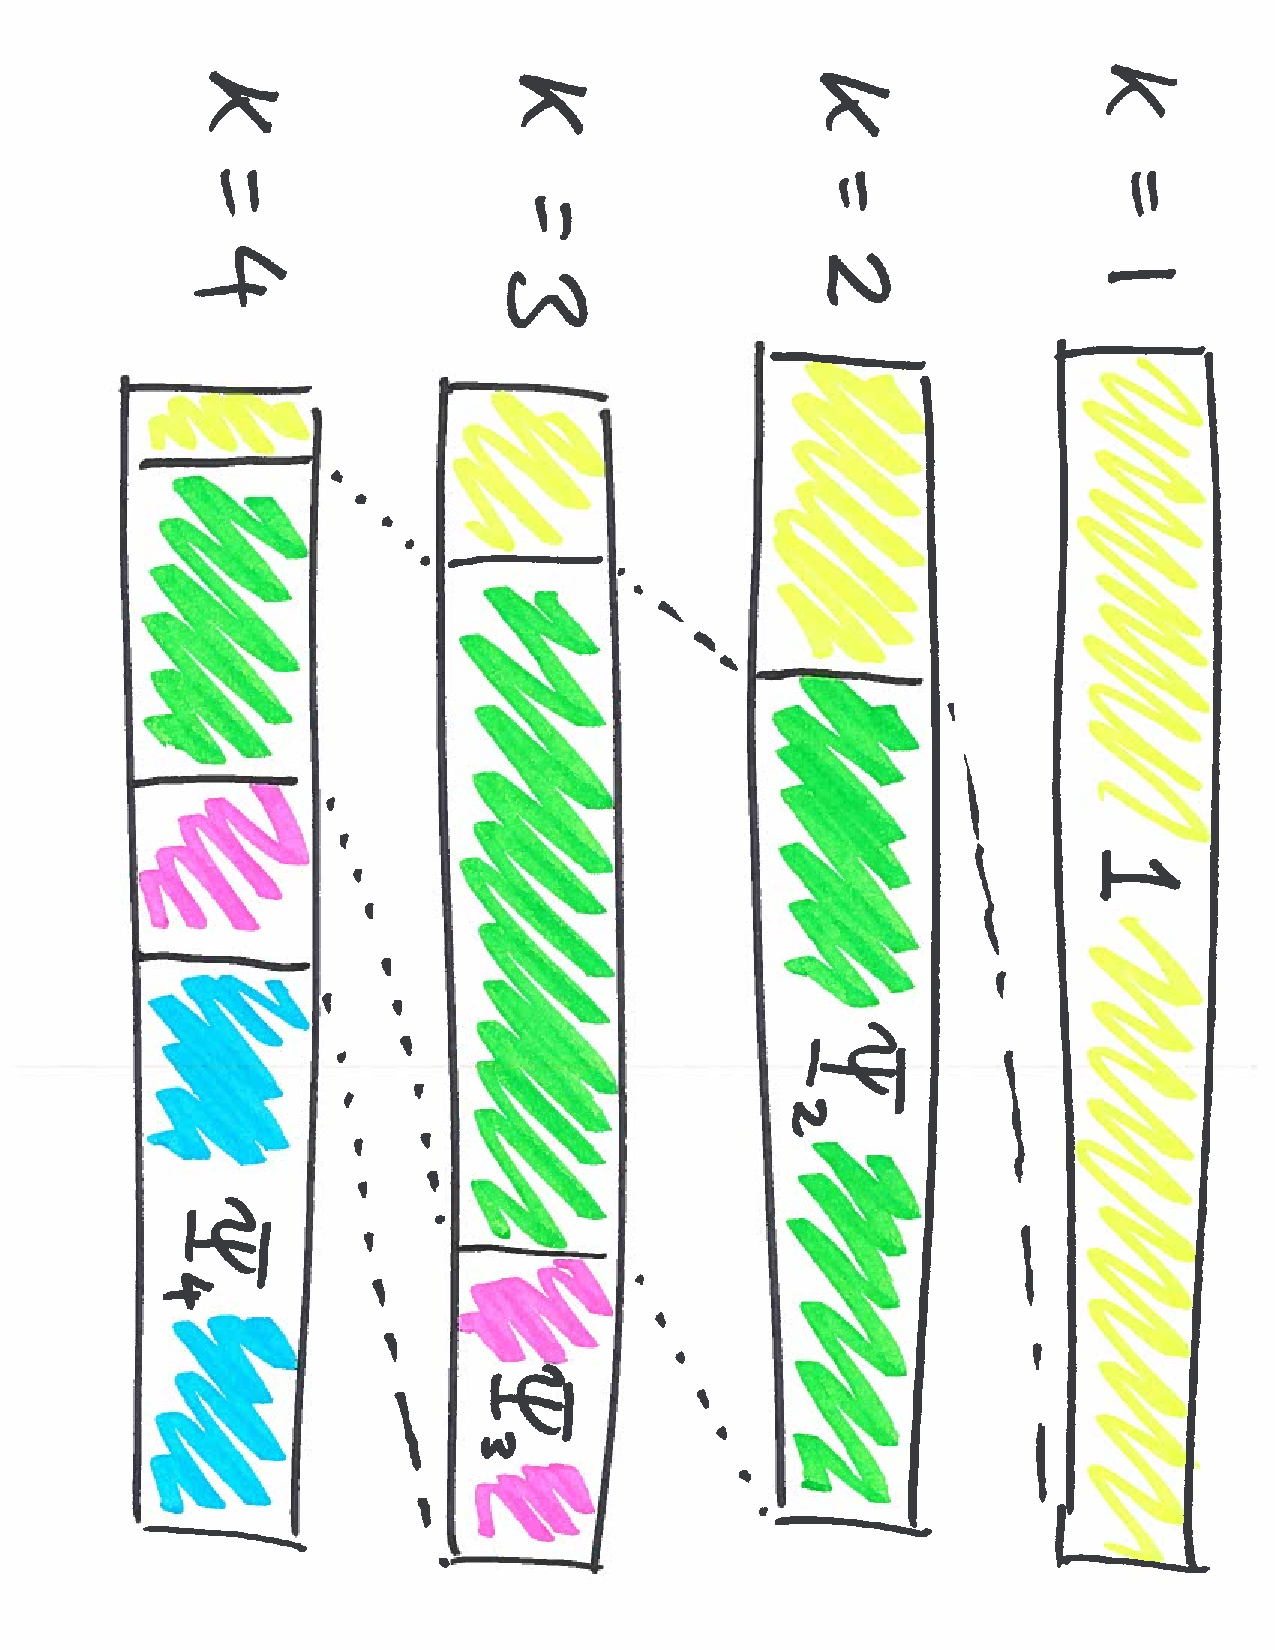
\includegraphics[angle=90,origin=c,scale=0.4]{fig/recursivescaling}
\end{frame}


\section{Sampling and inference}
\begin{frame}
	\frametitle{Sampling and inference}
	Why a paper on sampling and inference for BNTL models?
	\pause
	\begin{itemize}
		\item Inference is notoriously difficult for \textit{non-exchangeable} structures
		\item Need to identify \textit{exchangeable substructures}
	\end{itemize}
\end{frame}

\begin{frame}
	\frametitle{Exchangeable substructure}
	\begin{center}
		\resizebox{\textwidth}{!}{\begin{tikzpicture}[>=stealth]%[transform canvas={xshift=-0.5cm}]
    % \node[font=\scriptsize] at (-8.5,0.5) {$t$} ;
    % row 1
    \draw[shift={(-8.0,0)}] (-4pt,0) node[anchor=east,font=\scriptsize] {$1$} -- (4pt,0) {};
    % \draw[dotted,shift={(-8.0,0.0)},color=gray] (0,0) -- (8.0,0) {};
    \draw[densely dashed] (-8.0,0.5) node[anchor=south,font=\scriptsize] {$T_1=1$} -- (-8.0,-3.5) ;
    \foreach \x/\xtext/\xco in {0.0//red, 0.1//red, 0.2//red, 0.3//red, 0.6//red, 0.9//red, 1.3//red, 1.5//red, 1.7//red, 1.9//red, 2.2//red}
    	\fill[color=\xco] (-8.0+3*\x,0) circle (2pt) node[anchor=south,font=\scriptsize,color=black] {$\xtext$};
    \draw[densely dotted,color=red] (0.1,0.25) -- (-8.1,0.25) -- (-8.1,-0.25) -- (0.1,-0.25) ;
    % row 2
    \draw[shift={(-8.0,-1.0)}] (-4pt,0) node[anchor=east,font=\scriptsize] {$2$} -- (4pt,0) {};
    % \draw[dotted,shift={(-8.0,-1.0)},color=gray] (0,0) -- (8.0,0) {};
    \draw[densely dashed] (-8.0+1.2,0.5) node[anchor=south,font=\scriptsize] {$T_2$} -- (-8.0+1.2,-3.5) ;
    \foreach \x/\xtext/\xco in {0.4//blue, 0.5//blue, 0.7//blue, 0.8//blue, 1.1//blue, 1.4//blue, 1.8//blue, 2.1//blue, 2.4//blue}
    	\fill[color=\xco] (-8.0+3*\x,-1.0) circle (2pt) node[anchor=south,font=\scriptsize,color=black] {$\xtext$};
    \draw[densely dotted,color=blue] (-8.1+1.4,0.25) -- (-8.1+1.4,-1.25) -- (0.1,-1.25) ;
    % row 3
    \draw[shift={(-8.0,-2.0)}] (-4pt,0) node[anchor=east,font=\scriptsize] {$3$} -- (4pt,0) {};
    % \draw[dotted,shift={(-8.0,-2.0)},color=gray] (0,0) -- (8.0,0) {};
    \draw[densely dashed] (-8.0+3.0,0.5) node[anchor=south,font=\scriptsize] {$T_3$} -- (-8.0+3.0,-3.5) ;
    \foreach \x/\xtext/\xco in {1.0//green, 1.2//green, 2.3//green}
    	\fill[color=\xco] (-8.0+3*\x,-2.0) circle (2pt) node[anchor=south,font=\scriptsize,color=black] {$\xtext$};
    \draw[densely dotted,color=green] (-8.1+3.2,0.25) -- (-8.1+3.2,-2.25) -- (0.1,-2.25) ;
    % row 4
    \draw[shift={(-8.0,-3.0)}] (-4pt,0) node[anchor=east,font=\scriptsize] {$4$} -- (4pt,0) {};
    % \draw[dotted,shift={(-8.0,-3.0)},color=gray] (0,0) -- (8.0,0) {};
    \draw[densely dashed] (-8.0+4.8,0.5) node[anchor=south,font=\scriptsize] {$T_4$} -- (-8.0+4.8,-3.5) ;
    \foreach \x/\xtext/\xco in {1.6//magenta, 2.0//magenta}%, 2.4//magenta}
    	\fill[color=\xco] (-8.0+3*\x,-3.0) circle (2pt) node[anchor=south,font=\scriptsize,color=black] {$\xtext$};
    \draw[densely dotted,color=magenta] (-8.1+5.0,0.25) -- (-8.1+5.0,-3.25) -- (0.1,-3.25) ;
\end{tikzpicture}}
	\end{center}
\end{frame}

\begin{frame}
	\frametitle{Gibbs structure}
	The joint density has \textbf{Gibbs structure}
	\begin{equation*}
	p(\text{graph}|\bfT) = \prod_{j=1}^K p(\text{choose }j\ d_j\text{ times out of } n - T_j)
	\end{equation*}
	\begin{itemize}
		\item $K$ = \#vertices
		\item $n$ = \#edges
		\item $d_j$ = degree of vertex $j$
		\item $T_j$ = arrival time of vertex $j$
	\end{itemize}
\end{frame}

\begin{frame}
	\frametitle{Gibbs structure}
	Explicitly
	\begin{equation*}
	p(\text{graph}|\bfT) = \frac{\Gamma(d_1 - \alpha)}{\Gamma(n - K\alpha)}\prod_{j=2}^K \frac{\Gamma(T_j - j\alpha)\Gamma(d_j - \alpha)}{\Gamma(T_j - 1 - (j-1)\alpha)\Gamma(1-\alpha)}
	\end{equation*}
	\begin{itemize}
		\item $K$ = \#vertices
		\item $n$ = \#edges
		\item $d_j$ = degree of vertex $j$
		\item $T_j$ = arrival time of vertex $j$
	\end{itemize}
\end{frame}

\begin{frame}
	\frametitle{Available data}
	\begin{center}
		\begin{tabular}{ll}
			\textbf{Observation} & \textbf{Unobserved variables} \\
			\hline
			Entire history & $\alpha,\phi,\bfPsi$ \\
			Degrees in arrival order & $\alpha,\phi,\bfPsi, \bfT$ \\
			Snapshot & $\alpha,\phi,\bfPsi,\bfT,\sigma$
		\end{tabular}
	\end{center}
	\begin{itemize}
		\item $\alpha$ = BTNL parameter $\in (-\infty, 1)$
		\item $\phi$ = arrival distribution parameters
		\item $\bfPsi$ = latent sociabilities
		\item $\bfT$ = arrival times
		\item $\sigma$ = arrival order
	\end{itemize}
\end{frame}

\begin{frame}
	\frametitle{Gibbs sampler}
	\begin{center}
		\begin{tabular}{l|l}
			\textbf{Variable} & \textbf{Gibbs sampling scheme} \\
			\Xhline{4\arrayrulewidth}
			\rule{0pt}{3ex}
			$\alpha$ & MCMC, e.g. slice sampling \\
			\hline
			\rule{0pt}{3ex}
			$\phi$ & Depends on arrival dist. family $\Lambda_\phi$ \\
			\hline
			\rule{0pt}{3ex}
			$\mathbf{\Psi}$ & $\Psi_j | \text{graph}, \mathbf{\Psi}_{\setminus j} \sim \text{Beta}(d_{j} - \alpha, \bar{d}_{j-1} - (j-1)\alpha)$ \\
			& \quad where $\bar{d}_{j} = \sum_{i=1}^j d_{j}$ \\
			& \quad can marginalise out $\bfPsi$ \\
			\hline
			\rule{0pt}{3ex}
			$\mathbf{T}$ & Simple update for $T_j$, can't move past neighbours \\
			\hline
			\rule{0pt}{3ex}
			$\sigma$ & Initialise in descending degree order \\
			& \quad use M-H with adjacent swap proposal $\sigma_j \leftrightarrow \sigma_{j+1}$
		\end{tabular}
	\end{center}
\end{frame}

%\begin{frame}
%	\frametitle{Sampling $\bfPsi$}
%	Beta prior on $\Psi_j$, plus Gibbs structure, give
%	\begin{equation*}
%	\Psi_j \mid \text{graph}, \bfPsi_{\setminus j} \sim \text{Beta}(d_{j} - \alpha, \bar{d}_{j-1} - (j-1)\alpha) \;,
%	\end{equation*}
%	\small{where $\bar{d}_j = \sum_{i=1}^j d_i$}
%\end{frame}
%
%\begin{frame}
%	\frametitle{Sampling $\alpha,\phi$}
%	\begin{itemize}
%		\item One-dimensional unnormalized density for $\alpha$
%		\item For $\phi$ depends on arrival distribution family
%	\end{itemize}
%
%\end{frame}
%
%\begin{frame}
%	\frametitle{Sampling $\bfT$}
%	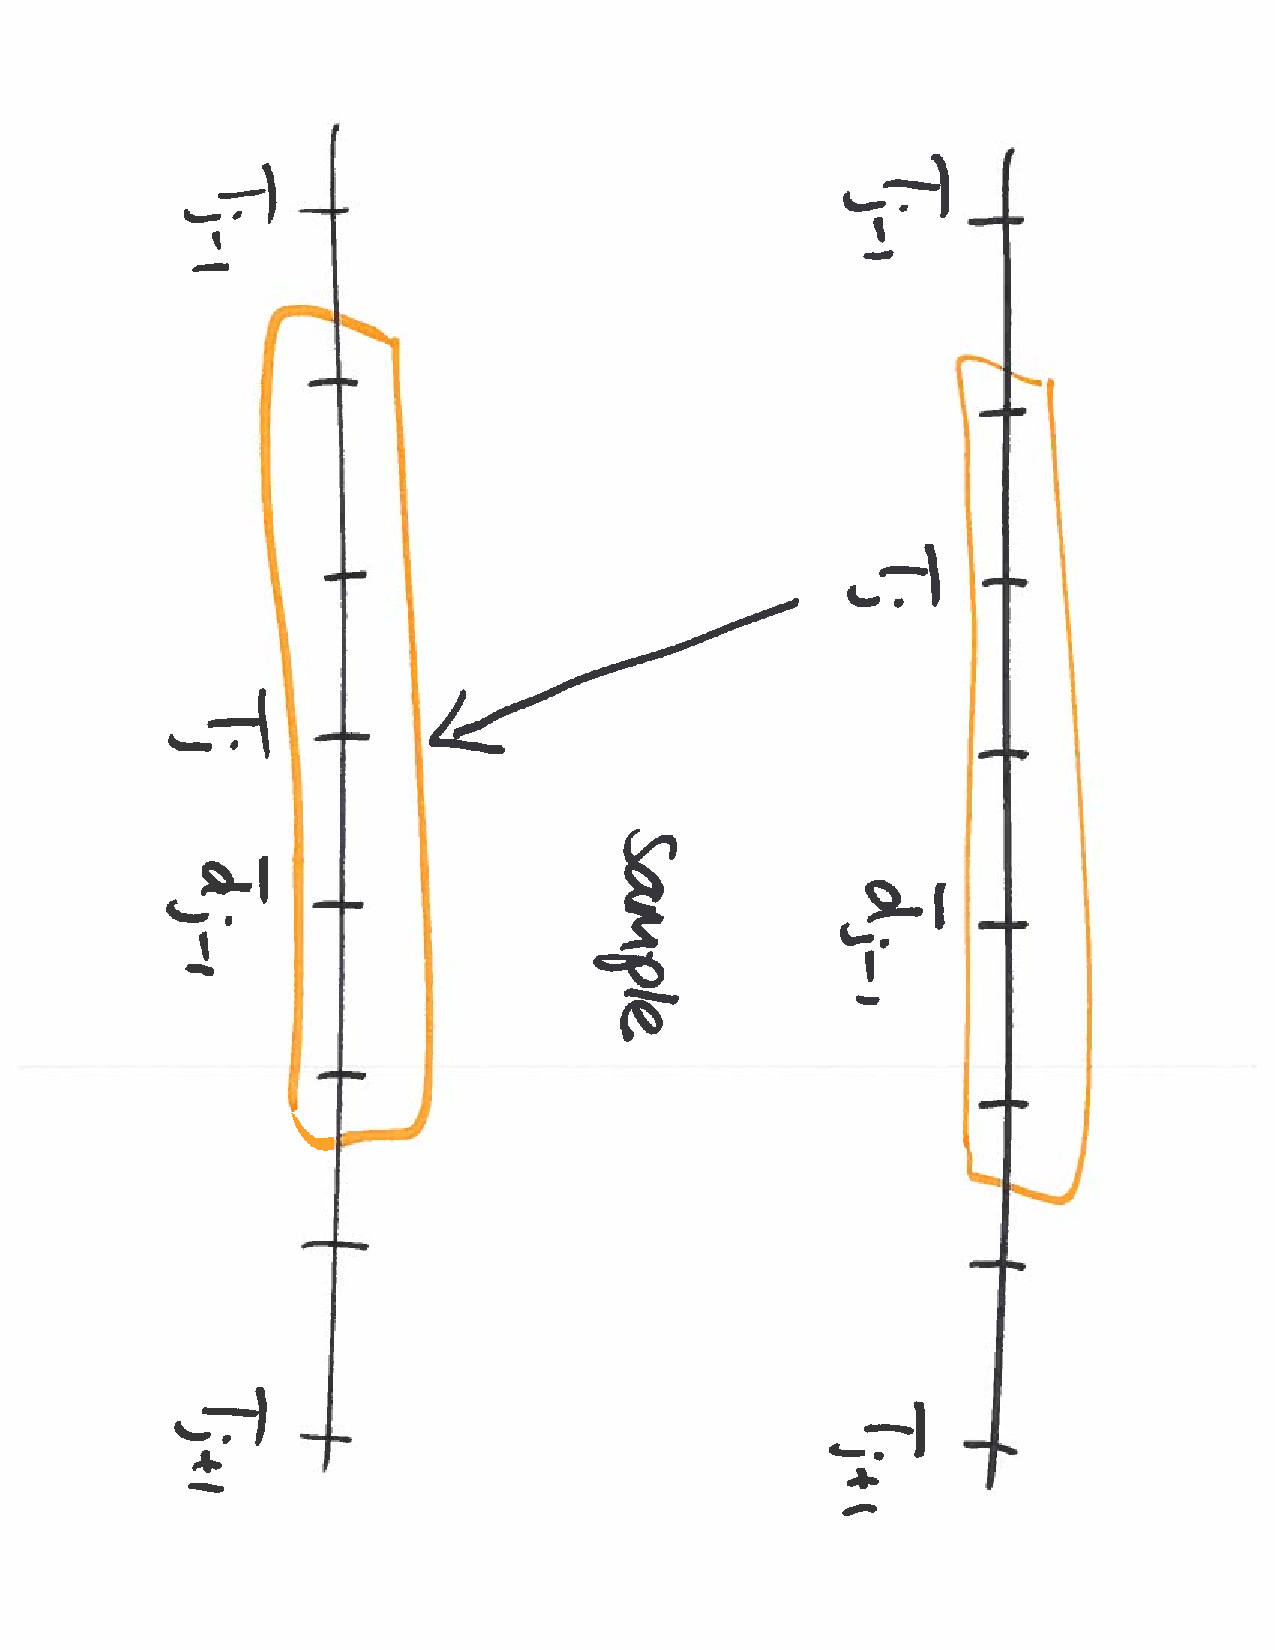
\includegraphics[angle=90,origin=c,scale=0.4]{fig/tsampling}
%\end{frame}
%
%\begin{frame}
%	\frametitle{Sampling $\sigma$}\
%
%	\begin{itemize} 
%	\item Initialise in descending degree order
%	\item Use Metropolis-Hastings with adjacent swap proposal $\sigma_j \leftrightarrow \sigma_{j+1}$
%	\end{itemize}
%\end{frame}

\begin{frame}
	\frametitle{Point estimation}
	If entire history observed,\textbf{maximum a posterior} (or \textbf{maximum likelihood}) estimates for $\alpha, \phi$ computable
\end{frame}

\section{Experiments}
\begin{frame}
	\frametitle{Experiments}
	\begin{itemize}
		\item Gibbs parameter recovery
		\item Gibbs scaling in $n$
		\item Point estimation with massive graphs
	\end{itemize}
\end{frame}

\begin{frame}
	\frametitle{Parameter recovery}
	\begin{itemize}
		\item Simulate 500 edges with fixed $\alpha$ 
		\item Arrivals either $\PYP$ or $\Geom$
		\item Observe final snapshot of the graph
	\end{itemize}
	\begin{table}[h]
		%  \caption{Results of Gibbs sampling experiments on synthetic data $(\alpha^* = 0.75)$. The top four rows show results from each of four different BNTL models fit to a synthetic graph with 500 edges generated by the coupled $\PYP$ BNTL model; the bottom four rows show the same BNTL models fit to a synthetic graph with $\Geom(0.25)$-distributed interarrivals.}
		\label{tab:ess}
		\vspace*{-0.75\baselineskip}
		\begin{center}
			\resizebox{1.0\textwidth}{!}{
				\begin{tabular}{lllll}
					Gen. arrival distn. & Inference model & $|\hat{\alpha} - \alpha^*|$ & Pred. log-lik.  \\
					\hline
					$\PYP(1.0,0.75)$ &  $(\tau,\PYP(\theta,\tau))$ &  \textbf{0.046 $\pm$ 0.002}   & -\textbf{2637.0 $\pm$ 0.1}  \\ 
					
					$\PYP(1.0,0.75)$  &  $(\alpha,\Geom(\beta))$  &  {0.049 $\pm$ 0.004} & -2660.5 $\pm$ 0.7  \\ 
					\hline
					
					$\Geom(0.25)$ & $(\tau,\PYP(\theta,\tau))$ &  0.086 $\pm$ 0.002   & -2386.8 $\pm$ 0.1  \\  
					
					$\Geom(0.25)$ & $(\alpha,\Geom(\beta))$ &  \textbf{0.043 $\pm$ 0.003}  & -\textbf{2382.6 $\pm$ 0.2}  \\ 
					
					\end{tabular}
					}
				\end{center}
			\end{table}
			
% where $\mathbf{S} := \frac{1}{K_n - 1} \sum_{j>1} (\bar{d}_{j-1} - T_j)$
\end{frame}

\begin{frame}
	\frametitle{Scalability of Gibbs sampler}
	\begin{itemize}
		\item Simulate with fixed $\alpha$ and $\Geom(\beta)$ arrivals
	\end{itemize}
	
	\begin{table}[t]
		\label{tab:ess:scale:n}
		\vspace*{-0.25\baselineskip}
		\begin{center}
			%  \resizebox{0.6\textwidth}{!}{
			\begin{tabular}{l  ll}
				& $100$ edges &  $10000$ edges \\ 
				\hline
				$|\hat{\alpha} - \alpha^*|$ & 0.12 $\pm$ 0.01 &  0.01 $\pm$ 0.00 \\ 
				
				$|\hat{\beta} - \beta^*|$ &  0.02 $\pm$ 0.00  &    0.00 $\pm$ 0.00  \\ 
				
				Effective Sample Size &  0.90 $\pm$ 0.04  &   0.75 $\pm$ 0.08  \\  
				
				Runtime (s) &  21 $\pm$ 0   &  2267 $\pm$ 2  \\ 
				
			\end{tabular}
			%}
		\end{center}
	\end{table}
	\begin{itemize}
		\item Most expensive Gibbs update is for $\bfT$
	\end{itemize}
\end{frame}

\begin{frame}
	\frametitle{MLEs for SNAP datasets}
	\begin{itemize}
		\item SNAP datasets
		\item Fit point estimates for $\alpha, \phi$
		\item Fit: coupled $\PYP$, uncoupled $\PYP$ and $\Geom(\beta)$ arrivals
	\end{itemize}
\end{frame}

\begin{frame}
	\frametitle{MLEs for SNAP datasets}
	Ask Ubuntu
	\begin{itemize}
		\item Estimates of $\PYP$ parameters vary significantly between coupled and uncoupled
		\begin{itemize}
			\item $\hat{\theta}, \hat{\alpha} = 18080, 0.25$
			\item $\hat{\theta}, \hat{\alpha}, \hat{\tau} = -0.99, -2.54, 0.99$
		\end{itemize}
		\item Edge exchangeable models misspecified ($\eta > 2$)
		\item Using $\Geom$ estimates $\eta$ well
	\end{itemize}
\end{frame}
	
%\begin{frame}
%	\frametitle{MLEs for SNAP datasets}
%	Though not for all datasets
%	\begin{table}[!ht]
%		\begin{center}
%			\color{lightgray}{
%				\resizebox{1.05\textwidth}{!}{
%					\begin{tabular}{llll | lllllll}
%						\multirow{2}{*}{Dataset} & \multicolumn{3}{c}{Coupled $\PYP(\theta,\alpha)$}  & &  \multicolumn{2}{c}{Uncoupled $\PYP(\theta,\tau)$} &  & \multicolumn{3}{c}{$\Geom(\geom)$}                             \\
%						\cline{2-4} \cline{6-7} \cline{9-11}
%						& $(\hat{\theta},\hat{\alpha})$ & $\hat{\eta}$           & Pred. l-l.            & $\hat{\alpha}$    & $(\hat{\theta},\hat{\tau})$ & Pred. l-l.     &     & $\hat{\beta}$  & $\hat{\eta}$   & Pred. l-l.                             \\
%						\hline
%						Ask Ubuntu  & (18080, 0.25) & 1.25   & -3.707e6              & -2.54            & (-0.99, 0.99)    & -3.678e6  &   &  0.083 & 2.32    & \textbf{-3.678e6}                         \\
%						UCI social network & (320.4, 4.4e-11) & --   & -1.600e5            & -4.98             & (5.50, 0.52)     & \textbf{-1.595e6}   &  & 0.016  & 2.10  & -1.596e5                    \\
%						EU email   & (113.6, 2.5e-14)  & --    & \textbf{-8.06e5}              & -1.86              & (113.6, 9.2e-10)      & \textbf{-8.06e5}  &   & 0.001  & 2.00   & -8.07e5                     \\
%						Math Overflow & (2575, 0.15) & 1.15  & -1.685e6              & -6.62           & (-0.97, 0.997)    & -1.670e6 &    & 0.025  & 2.19   & \textbf{-1.670e6}                \\
%						Stack Overflow & (297600, 0.11) & 1.11 & -3.358e8             & -8.94            & (-1.0, 1.0)      &  -3.333e8  &    &  0.020  & 2.21   & \textbf{-3.333e8}                 \\
%						Super User  & (20640, 0.24) & 1.24  & -5.855e6            & -4.19          & (-0.996, 1.0)      &  \textbf{-5.775e6}   &  & 0.067 & 2.37    & -5.775e6              \\
%						Wikipedia talk pages  & (14870, 0.54) & 1.54  & -3.074e7          & -0.25            & (-1.0, 1.0)   & \textbf{-3.066e7}  &   & 0.073  & 2.10   & -3.066e7                   
%					\end{tabular}
%				}}
%			\end{center}
%			\vspace*{-\baselineskip}
%		\end{table}
%	\end{frame}

\begin{frame}
	\frametitle{Conclusion}
	\begin{itemize}
		\item BNTL models are \textit{flexible}
		\item BNTL models are \textit{tractable}
	\end{itemize}
\end{frame}

\begin{frame}
	\frametitle{Future work}
	\begin{itemize}
		\item Scalability of inference
		\begin{itemize}
			\item Metropolis-Hastings to update $\bfT$ altogether
			\item Variational inference for $\sigma$
		\end{itemize}
	\end{itemize}
\end{frame}

\begin{frame}
	\frametitle{References}
	\tiny{\bibliographystyle{unsrt}
	\bibliography{refs}}
\end{frame}

\end{document}
